\chapter{Reliable Visualizations}\label{chap5}

Text

\section{Introduction}

Flow visualization has been around in some form for as long as people have studied flows.  In some
cases, visualization was done explicitly -- that is, with the expressed purpose of the viewer to highlight
some feature of the flow.  In other cases, it was done tacitly, as when a child looks out the window
of an airplane to see the slip-stream over the wing generated upon take-off.  Visualization has
many roles, spanning from art to science.  In this work, we focused on visualization techniques
used for the scientific exploration and explanation of flow phenomena.  In particular, we are interested
in how two communities -- the AIAA community and the Visualization community -- consider
flow visualization.  To accomplish this task, we have used the {\em AIAA Journal} and the
{\em IEEE Transactions on Visualization and Computer Graphics (TVCG)} as ``representative" publication
venues of the two communities, and have explored the papers published therein to try to 
glean how each community approaches visualization of flow, how they might differ from each other 
and how the two communities might complement each other. 

This work is organized as follows.  In Section \ref{sec:flowvis} we provide a review of the state-of-the-art
in flow visualization, both from the perspective of the Visualization and well as the AIAA communities. 
%
Tools such as Tecplot\cite{amtec1996tecplot} and Paraview\cite{squillacote2007paraview} have implemented many 
standard flow visualization techniques such as LIC (line integral convolution), streamlines, stream ribbons, and more. 
As we will show, our review encompasses much of the current practices in 
flow visualization and also provide pointers to new developments. 
%
In the next two sections, we focus our attention on research advances made within the Visualization 
community that we think will, in time, have impact on flow visualization and on other application domains
that use visualization as a means of both scientific exploration and explanation.  
In Section \ref{sec:perceptionandevaluation} we show how perception and user studies may impact flow visualization, and
in particular, we focus on
issues related to color maps.  In Section \ref{sec:verif}, we then provide
discussions on the current Visualization community research trends in Visualization Verification 
and Uncertainty Quantification.  We have chosen these topics because they are all related to flow visualization.
%In Section \ref{sec:tools} we review the set of currently
%available tools to fluids researchers, highlighting that some of these tools in fact have some of the
%advanced features of the Visualization Community, even if the general user-base is not aware.
In Section \ref{sec:opportunities}, we speculate on some of the opportunities for collaboration and
more effective communication between the two communities, and we conclude in Section
\ref{sec:conclusions}.

\begin{table}
\caption{\label{table:progress}Advances in flow visualization. This table is \emph{not} meant to be comprehensive.}{}\centering
\begin{tabular}{c c r p{8.5cm}}
\toprule
Class &  Subclass & Technique & Reference\\
\hline
\multirow{5}{*}{\bf Direct} 	&\multirow{4}{*}{\em Arrows}		& \cc Standard  & \cc Klasshen and Harrington\cite{Klassen:1991:SHT:949607.949631} \\
					&							& \cc Hybrid  	& \cc Color-coding and arrows\cite{Kirby:1999:VMD:319351.319429}\\
					&							& \cc 3D  			& \cc Arrows in 3D space, 2-manifolds embedded in 3D\cite{Peng:2012:MVF:2086335.2086624}\\
					&							& \cc Enhancements& \cc Large data\cite{Peng:2012:MVF:2086335.2086624}, resampling\cite{Laramee2003905}\\
					&\multirow{1}{*}{\em Color coding}	&  Standard	&  Color maps, volume rendering\cite{Engel:2004:RVG:1103900.1103929}\\
\hline
\multirow{8}{*}{\bf Geometry}	&\multirow{5}{*}{\em Curve}	& \cc Streamline  	& \cc Turk and Banks\cite{Turk:1996:ISP:237170.237285}\\
						&						& \cc Seeding		& \cc User-assisted\cite{Jobard97creatingevenly-spaced}, automatic\cite{MebarkiAD05,li2008illustrative}, and hierarchical\cite{jobard2001multiresolution}\\
						&						& \cc 3D			& \cc 2-manifolds embedded in 3D\cite{spencer2009evenly}\\
						&						& \cc Rendering	& \cc Illuminated\cite{Mattausch:2003:SIE:984952.984987}, streamtubes and streamribbon\cite{Ueng:1996:ESS:614262.614333}\\
						&						& \cc Unsteady		& \cc Wiebel and Scheuermann\cite{wiebel2005eyelet}\\
						&\multirow{3}{*}{\em Surface}	& Stream surface  	& Hultquist\cite{Hultquist:1992:CSS:949685.949718}\\
						&						& Enhancements	& Seeding and placement\cite{Peikert:2009:TRS:1980462.1980472}, accuracy\cite{Garth:2008:GAI:1477066.1477441}\\
						&						& Unsteady		& Schafhitzel \emph{et al.}\cite{Schafhitzel:2007:PSS:1268517.1268564}\\
\hline
\multirow{8}{*}{\bf Texture}&\multirow{5}{*}{\em LIC}		&\cc Standard		&\cc Cabral and Leedom\cite{Cabral:1993uu} \\
					& 							&\cc Performance	&\cc Improved algorithm, parallelism, real-time, GPU\cite{Li:2006:GIA:2384796.2384800}\\
					& 							&\cc 3D			&\cc 3D and 2-manifolds embedded in 3D\cite{10.1109/TVCG.2010.121}\\
					& 							&\cc Rendering		&\cc Flow orientation cues, local velocity magnitude\\
					& 							&\cc Unsteady 		&\cc Li \emph{et al.}\cite{Li:2006:GIA:2384796.2384800}\\
					&\multirow{3}{*}{\em Spot Noise}	& Standard			& van Wijk\cite{vanWijk:1991vd} \\
					& 							& Enhanced 		& It deals with highly curved/high velocity vector fields.\cite{deLeeuw:1995tp} \\
					& 							& Performance		& Parallel implementation.\cite{Leeuw:1997vr} \\
\hline
\multirow{6}{*}{\bf Feature}	&\multirow{4}{*}{\em VFT$^{*}$}	&\cc Standard		&\cc First-/High-order critical point tracking\cite{Helman:1989:RDV:72885.72887,de1999visualization,Scheuermann:1998:VNV:614270.614397} \\
						& 							&\cc Compression 	&\cc Theisel \emph{et al.}\cite{CGF:CGF680}\\
						&							&\cc Simplification	&\cc Weinkauf \emph{et al.}\cite{weinkauf05a}\\
						& 							&\cc Streakline 		&\cc Weinkauf and Theisel \emph{et al.}\cite{Weinkauf:2010:SLT:1907651.1908009}\\
						&\multirow{1}{*}{\em STD$^{**}$}	& Pathline			&Theisel \emph{et al.}\cite{Theisel:2005:TMT:1070610.1070741} \\
						&\multirow{1}{*}{\em LM$^{***}$}	&\cc FLTE			&\cc Haller\cite{Haller:2001:DMS:370169.370176},  Garth \emph{et al.}\cite{Garth:2007:ECV:1313046.1313106}\\
\hline
\multicolumn{4}{l}{$^{*}$ Vector Field Topology $^{**}$ Space-Time Domain $^{***}$ Lagrangian Method}\\
\bottomrule
\end{tabular}
\end{table}

%%%%%%%%%%%%%%%%%%%%%%%%%%%%%%%%%%%%%%%%%%%%%%%%%%%%%%%%%
\section{Review of Flow Visualization Techniques}
\label{sec:flowvis}

%* Intro
%* Review of flow vis 
%	- Vis community
%	- AIAA community
%* How mature is the flow vis field? Evaluation, Uncertainty, and Verification of flow vis techniques.
%      - Here we show a plot of the new wave of evaluation papers/user studies inside the Vis community
%* Opportunities:
%	- Does the Vis community knows the problems and challenges faces by AIAA community?
%	- Does the AIAA community knows the advances made by the Vis community?

Vector field visualization is an important and vibrant subfield of both the Visualization and AIAA communities.
%
The techniques developed for vector field visualization extend beyond these communities to fields such as medical imaging, meteorology, the automotive industry, and others.
%
In the past two decades, visualization experts and practitioners have seen the development and improvement of many vector field visualization techniques.
%
The contributions are numerous: the ability of handling different grid types (structured, unstructured, curvilinear, etc), high dimension data (2D, 2.5D, and 3D), time-dependent flow, seeding and placement of geometric primitives, improved performance, perception, rendering, among others.
%
In this section, we review some of the developments inside the Visualization community and compare with current practices inside the AIAA community.

\subsection{Preliminaries}

Although the concept of flow visualization is well defined in both communities, we start by clarifying what is meant by flow visualization in this section.
%
The difference between \emph{computational flow visualization} and \emph{flow visualization} is that the latter focus on visualization of flow behavior using experimental data (\emph{e.g.}, flow in a wind tunnel), whereas the former visualizes flow from simulated or computed data. 
%
Some computational visualization techniques are inspired by techniques used in flow visualization, such as dye advection. 
%
Since the subject of this section only addresses computational flow visualization, we will refer to that topic simply as flow visualization.

For thoroughness, we also define some commonly used mathematical/physical terms used within the flow visualization literature.
A \emph{streamline} is the path traced by a massless particle in a steady flow. Streamlines are sometimes referred to as ``instantaneous particle trace''.
%
A \emph{streakline} is the path traced by massless particles seeded at the same position but at different times in a unsteady flow. 
%
\emph{Stream surfaces} and \emph{streak surfaces} are the 2-manifold analog of streamlines and streakline, where the seeding primitive is a curve instead of a point.

\subsection{Classes of techniques}

Flow visualization techniques can be classified as direct, geometric, texture-, and feature-based. 
%
Table \ref{table:progress} provides an overview of the classification and a subset of the available techniques within each class.  
%
The table provides a hierarchy of the flow visualization tools available.
%
The \emph{Subclass} column provides the main component of a given visualization techniques that can be found within the \emph{Technique} column.
%
One can find reference to extra material within the \emph{Reference} column. 
%
For more details about the articles shown in Table \ref{table:progress} and others, we refer the interested reader to the excellent surveys by Hauser \emph{et al.}\cite{Hauser:2003tm} and Peng and Laramee\cite{peng2009higher} for an overview of the flow visualization field, Edmunds \emph{et al.}\cite{Edmunds2012974} and McLoughlin \emph{et al.} \cite{CGF:CGF1650} for geometric flow visualization, Laramee \emph{et al.}\cite{laramee2004state, laramee2008applications} for texture-based flow visualization, and Pobitzer \emph{et al.}\cite{CGF:CGF1901} for feature-based flow visualization. 
%
Next, we briefly go over each of the classes (see Figure \ref{fig:classes}).

\begin{figure}[ht]
\centering

\includegraphics[width=1\linewidth]{chapter6/figures/classes.png}
\caption{Examples of flow visualization using direct, geometry, texture-, and feature-based techniques, respectively.}
\label{fig:classes}
\end{figure}

%%%% Direct visualization
\paragraph{Direct visualization} 
%
Direct visualization techniques provide an intuitive and straightforward way of visualizing vector fields. 
%
In this approach, primitives of interest -- such as arrows, glyphs, or lines -- are placed at (often regularly-spaced) seed points. 
%
The primitives are then oriented according to the vector field. 
%
Optionally, the vector magnitude can be mapped to the primitives via scaling. 
%
%Although the research into direct visualization has slowed down in recent years, the work by Peng \emph{et al.}\cite{Peng:2012:MVF:2086335.2086624} is a recent development combining vector field clustering for unstructured grid and glyph placement on boundary surfaces. 
%
Other flow properties, such as pressure and vorticity, can also be mapped using color maps.
%
In the 3D case, volume rendering\cite{Engel:2004:RVG:1103900.1103929} is the natural choice for mapping flow properties into color and transparency.
%
Although direct visualization provides an easy first approximation of the vector field, the visual complexity and occlusion may impair the interpretation of the results, especially in 3D datasets.

%%%% Geometric visualization
\paragraph{Geometric visualization} 
%
In geometric visualization, curves and surfaces are used for summarizing flow behavior at particular seed points.
%
Geometry-based approaches requires a more intensive processing of the data before the visualization than direct approaches. 
%
The main idea behind integration-based geometric flow visualization is to trace particles or curves through the vector field. 
%
By tracing particles (or respectively curves) one builds a 1-manifold (or respectively a 2-manifold) that can later be visualized.
%
Geometric visualization techniques have a two steps: first, geometry computation; and secondly, rendering. 
%
Often, the rendering step is straightforward -- \emph{e.g.} rendering a polyline -- in which case the algorithm collapses into one step.
%
Streamlines are one of the most well-known representative visualization tools within this class. 
%
Although flow visualization using both curves and surface dates back over two decades, in recent years there has been constant research on the topic\cite{Edmunds2012974}. 
%
%Some of the challenges that have been tackled are the problems of occlusion, seeding and placement of primitives, and rendering.
%
% Curves
For curves, the main contributions of the past decade are related to rendering, seeding and placement of curves.
%
% Surface
Edmunds \emph{et al.}\cite{Edmunds2012974} classifies the surface-based flow visualization into surface construction and rendering. 
%
Methods for surface construction are based on integral surface, implicit and topological construction. 
%
This is an area of intense research in the past few years.
%
The authors present a variety of algorithm for both steady and time-dependent surfaces. 
%
Surface rendering methods involve the use of several techniques for improving the quality of the visualization of the flow over a surface of interest. 
%
Surface-based techniques can take advantages of direct or texture-based methods by including static/animated arrows over stream surfaces, shading for the evaluation of the shape of surfaces, placing streamlines over 3D surfaces, employing line-integral convolution (LIC) techniques, and/or non-photorealistic rendering techniques.

%%%%% Feature-based visualization
\paragraph{Feature-based visualization} 
%
In feature-based flow visualization, the input vector field is segmented according to features of interest. 
%
As an example, consider a segmentation using classical vector field topology in 2D\cite{Helman:1989:RDV:72885.72887} (see also the right image in Figure \ref{fig:classes}). 
%
Let us assume that the features of interest are first order critical points, namely, focus source, focus sink, node source, node sink, and saddles. 
%
A segmentation is performed by building a topological skeleton through the computation of the vector field's separatrices.
%
The final result provides a cleaner representation of the flow behavior in terms of the aforementioned features.
%
The intensive processing of extracting features before visualization brings many advantages to the practitioner.
%
First, feature-based techniques are valuable for visualization purposes: 
%
feature extraction provides an excellent level of abstraction of the data by removing undesired features and focusing the viewer on the important regions of the dataset.
%
In addition, it can be used for vector field compressing, topological simplification, and even for building custom vector fields\cite{theisel2008}. 
%
Topology-based approaches for feature-based visualization is not the only methodology available.
%
In Lagrangian methods, the trajectories of particles are used to describe and segment the fluid flow.
%
In particular, FLTE\cite{Haller:2001:DMS:370169.370176} methods have gained prominence as a research area within the last decade.
%
One advantage of Lagrangian methods over traditional vector field topology is that they can naturally deal with unsteady flow\cite{CGF:CGF1901}. 
%
Space-time domain techniques are another example of feature-based visualization.
%
In this approach, in order to deal with the problems involved in unsteady flows, the problem of 2D and 3D flow visualization is moved to higher dimensions.
%
As an example, time-dependent domains are merged into a single dataset where traditional techniques used for steady vector fields can be employed.
%
A comprehensive survey on the topic can be found in the state-of-the-art report by Pobitzer \emph{et al.}\cite{CGF:CGF1901}.


%%%%% Texture-based visualization
\paragraph{Texture-based visualization} 
%
In texture-based flow visualization, the user replaces geometrical information with 2D texture mapped over surfaces. 
%
Line integral convolution (LIC) is a well-known (within the visualization community, at least) representative of the class. 
%
Texture-based techniques generate what is considered a dense visualization, \emph{i.e.}, it covers the entire domain of interest,
%
%\footnote{This is not ideal for all kinds of tasks, as suggested in previous user study where participants performed worse when using LIC\cite{cite study where LIC performs worse than other 2D flow vis}}
%
and it does not have to deal with the problem of finding appropriate seeding spots for streamlines. 
%
Texture-based techniques can be applied along with geometric or feature-based visualization; for instance, it can be used to render flow on 2-manifolds embedded in 3D spaces, or providing an overview of the flow behavior along with topological skeletons.
%
The main issue with texture-based visualizations is the high computational cost associated with it. 
%
Nevertheless, the advances in both computer hardware and algorithms have granted to users the ability to handle large data sets and unstructured grid at interactive rates\cite{Edmunds2012974, laramee2008applications}.

\subsection{Means to an end}
%% Stats:
%Grid Type Used: Cartesian, Unstructured, Curvilinear, B-Spline Volumetric Mesh, Quad-tree
%Domain: 2D, 3D, and 2-manifold embedded in 3D space
%Papers containing at least one flow visualization technique: 78
%2D Contour and 2D color maps were left out because they appear in too many papers
%3D streamlines/streamtrace/pathline: 15	
%2D streamlines/streamtrace/pathline: 33
%3D Contour: 27
%2D Glyphs/Arrows: 24
%3D Glyphs: 2
In his position paper ``On the death of visualization''\cite{citeulike:4186603}, Lorensen argues for the need to bring visualization researchers closer to experts and practitioners. 
%
We have run a simple experiment in order to attempt to ascertain ``the distance" between the Visualization and AIAA communities.
%
We evaluated 78 articles published within the {\em AIAA Journal} over the period of Jan/2010-Oct/2012 containing at least one flow visualization image. 
%
Then, we simply counted the number of papers that contained at least one occurrences of the techniques shown in Table \ref{table:progress}. 
%
We did not include the 2D color mapping and 2D isocontour visualizations as they appear quite often. 
%
Since multiple visualization techniques can be used in a single article, the percentages shown below are just the fraction of publications containing at least one particular type of visualization.
%
Particle tracing using integration-based geometric visualization techniques for 2D vector fields is the most commonly used technique ($42\%$), followed by 3D isocontouring ($35\%$), 2D and 3D arrows and glyphs ($33\%$), and 3D particle tracing ($19\%$). 
% 
Excluding isocontouring (which is mainly used for depicting scalar, instead of vector, data), $61\%$ of the articles used at least one geometric approach to flow visualization, whereas $33\%$ used a direct approach. 
%
Finally, $73\%$ of the papers contained at least one visualization for 2D domains, whereas this number is $56\%$ for 3D domains. 
%
The latter number drops to $22\%$ if one considers only techniques for visualization of vector field data (\emph{i.e.}, excluding 3D isocontouring).

Although the data is limited to a short window of time, it raises a few interesting points. 
%
With the exception of a handful of papers, most of the flow visualization appears to be using the standard form of the traditional visualization technique.
%
As an example, consider some the papers that use streamlines for visualizing 3D flow. 
%
It may be the case that a subset of these paper can benefit from using stream ribbons\cite{Ueng:1996:ESS:614262.614333}, which simultaneously encode the streamlines path and local flow vorticity,
%
or from stream tubes\cite{Ueng:1996:ESS:614262.614333}, which simultaneously encode the streamlines path and local cross flow divergence. 
%
Both stream ribbons and stream tubes are well-known, and commonly used visualization packages such as Paraview or Tecplot have them available within their tool options.
%
%
%
%
Secondly, the preference for the two visualization techniques (direct and curve-based geometric visualization) shown in past three years is perhaps due to their simplicity and availability. 
%
The underrepresented methods in the same period of time are texture-, feature-, and surface-based flow visualization.
%
%
%
%
%
Third, one could argue that the visualized datasets were ``simple'', and thus standard techniques worked well. 
%
Even though this may be the case for some datasets, some vector fields, especially in 3D, suffered from traditional problem of curves and arrows:
%
cluttering, irregularly spaced streamlines, poor seeding, lack of depth cues,  {\em etc.} 
%
These problems can make the detection of some flow features such as vortex more difficult. 
%
Direct visualization for 2D vector fields using glyphs can be improved by using, for instance, a resampling technique, such as shown in Laramee\cite{Laramee2003905}, where the author introduce a user-driven approach for reducing visual clutter via resampling. 
%
Another way is to segment the flow using features of interest, \emph{e.g.} critical points.
%
%
%
%
%
%
%
Possible reasons for \emph{not} using alternative techniques include that the technique might not be easily available, the technique might not improve the quality of the visualization, users not aware of their existence or find them difficult to use, or the AIAA community 
requires a different class of techniques, among other.
%
%
Both communities would benefit from knowing the reasons for using one technique over another.  
%
The visualization community has, throughout the years, defined a set of priorities based on an interaction with researchers from different fields and their own experience.
%
Some recurrent themes that are the focus of research are: 
%
a more comprehensive theory and techniques for dealing with unsteady 3D flows; 
%
improved rendering (for instance, by using techniques inspired in handcrafted illustrations\cite{Brambilla12Illustrative});
%
handling of large data sets; and others.
%
Together, the AIAA and Visualization communities should be 
able to define a set of priorities for their research agendas 
in order to address the concerns and issues raised.



%%%%%%%%%%%%%%%%%%%%%%%%%%%%%%%%%%%%%%%%%%%%%%%%%%%%%%%%%%%%%%%%%%%%
\section{Perception and Evaluation}
\label{sec:perceptionandevaluation}

An important aspect of the visualization research consists of the building of new visualization techniques and tools.
%
Ideally, new techniques should be able improve the user cognitive process\cite{Tory:2004:HFV:951847.951892}, for instance, by allowing the visualization of data that has never been visualized before, or increasing ones ability to interact with, understand, and explore data.
%
As visualization techniques are developed and improved, a question is raised: how can we compare and understand the differences between visualization techniques?
%
The answer to this question leads us to a second important research topic:
%
the need for rigorous evaluation of the strengths and weaknesses of visualization techniques.
%
By ``strength'' and ``weakness'' we mean not only the evaluation of techniques according to traditional (computer science) metrics such as performance, memory footprint, ability to handle large datasets, {\em etc.}, but also in terms of the errors introduced through visualization, property of these errors, user perception, among others.
% 
In particular, questions involving perception and cognition are related to the \emph{user}.
%
In this section, we review two topics of interest for flow visualization from the point of view of  perception and evaluation: the use of color maps for visualization of scalar properties and the representation of steady 2D vector fields, respectively.

\subsection{Perception \& color maps}

%	Introduction to the importance of color map;
%
%	Damage caused by the rainbow color map;
%		- Explain the problem with ordering, isoluminance, and perceived gradients;
%		- Examples;
%		
%		- Problems caused by rainbow colormap in areas such as medicine;
%		- Paraview's repentance;
%	
%	Review of the situation inside the AIAA journal; 
%		- Statistics collected from the papers published in the last two years
%		- Can we improve some of these images?
%	
%	Conjecture on possible damage caused by RCM to the AIAA community;
%	Examples would be very nice;
%	
%	Alternatives to rainbow colormap: what are the recommendation for visualizing colors on surface, 
%	
%	Possible collaboration between communities

The mapping between data and colors is ubiquitous and essential across the sciences. 
%
In the scientific pipeline, color maps are often used to study, explain, explore, and ultimately help 
experts to gain insight about a phenomenon of interest. 
% 
Alas, color maps are not all equal, and depending on the choices made one can accelerate or 
impair scientific inquiry. 
%
Since they are just means-to-an-end, their impact on the underlying data should be as minimal as possible.
%
In a myriad of choices, one color map has been shown to be a bad choice for virtually any type of 
visualization: the well-known and widely-used \emph{rainbow} color map.\cite{Borland:2007:RCM:1251554.1251614, 
macdonald1999using, Silva2011320}. 

The rainbow color map is built by varying hue in order to cover the whole spectrum of visible light, 
from red to purple or vice versa. In practice, many visualization tools use colors varying from red to blue because red and purple are very similar.
%
It is the default map in several visualization / simulation software packages, such as Matlab\textsuperscript{\textregistered}.  
%
Here we review three issues known to hinder visualizations, namely, lack of ordering, iso-luminance, 
and introduction of artifacts. 
%
 \begin{figure}[tp]
 	\centering
       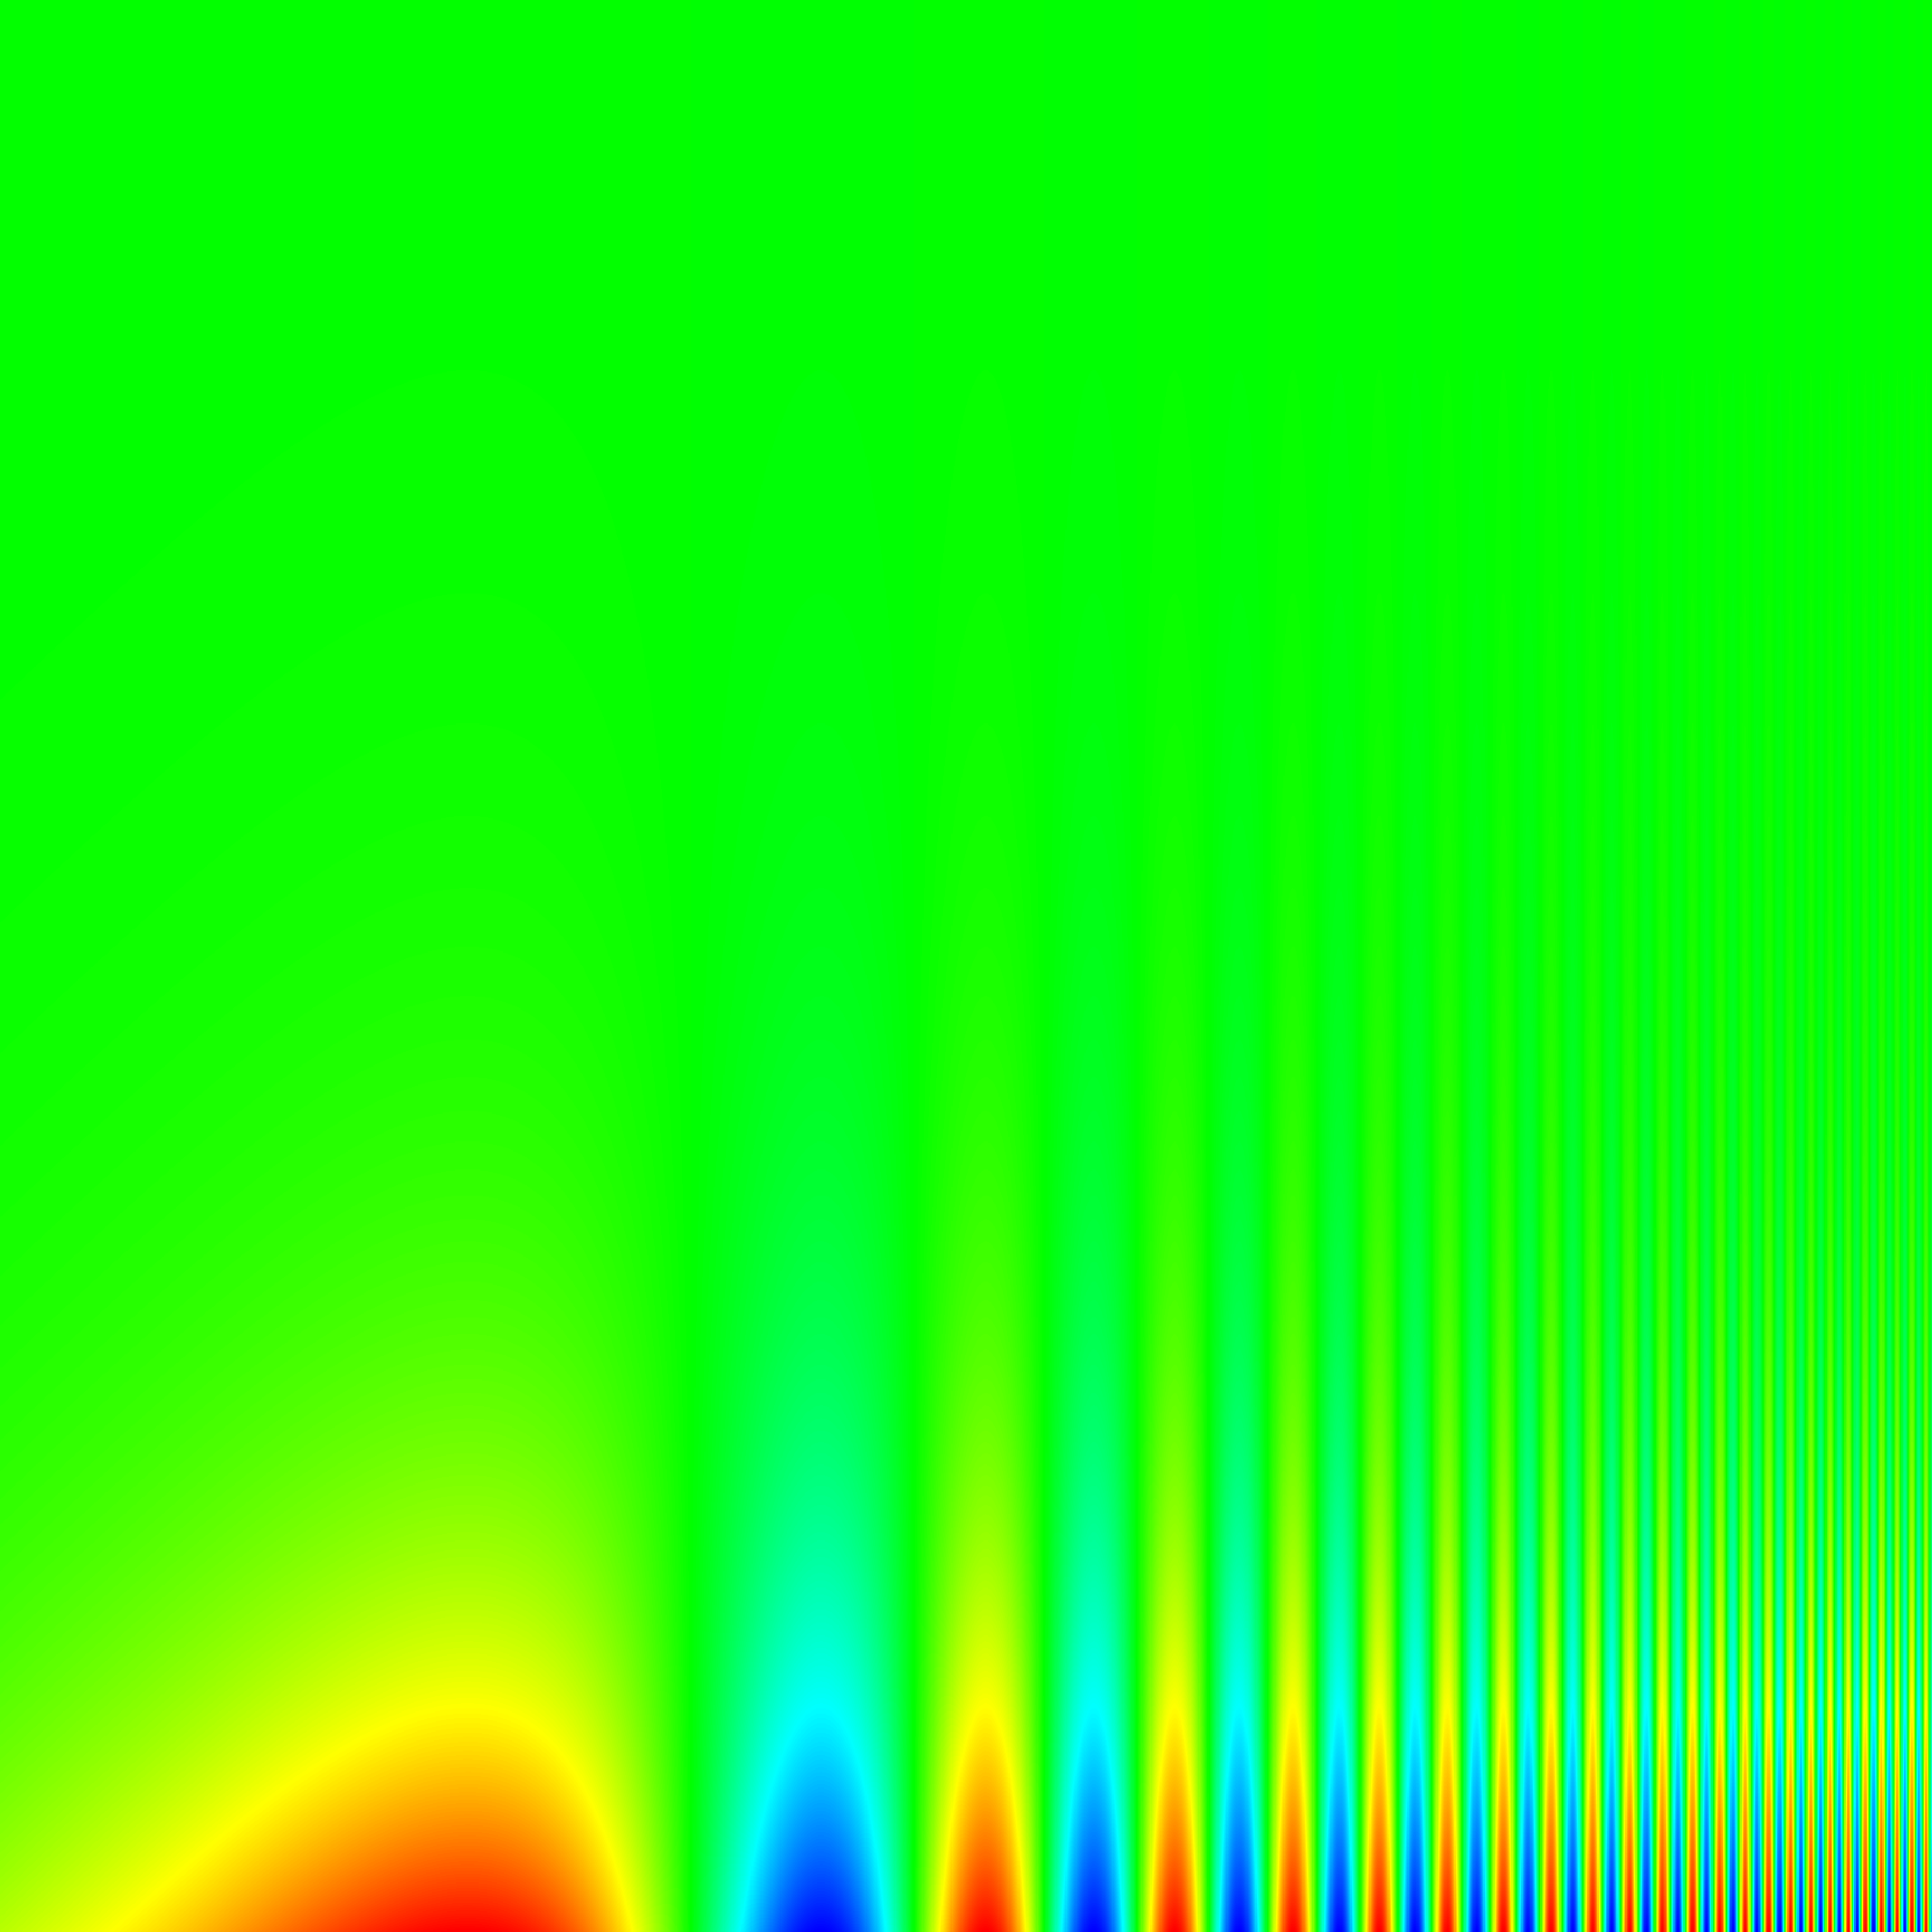
\includegraphics[width=0.235\linewidth]{chapter6/figures/scsf-rainbow}
       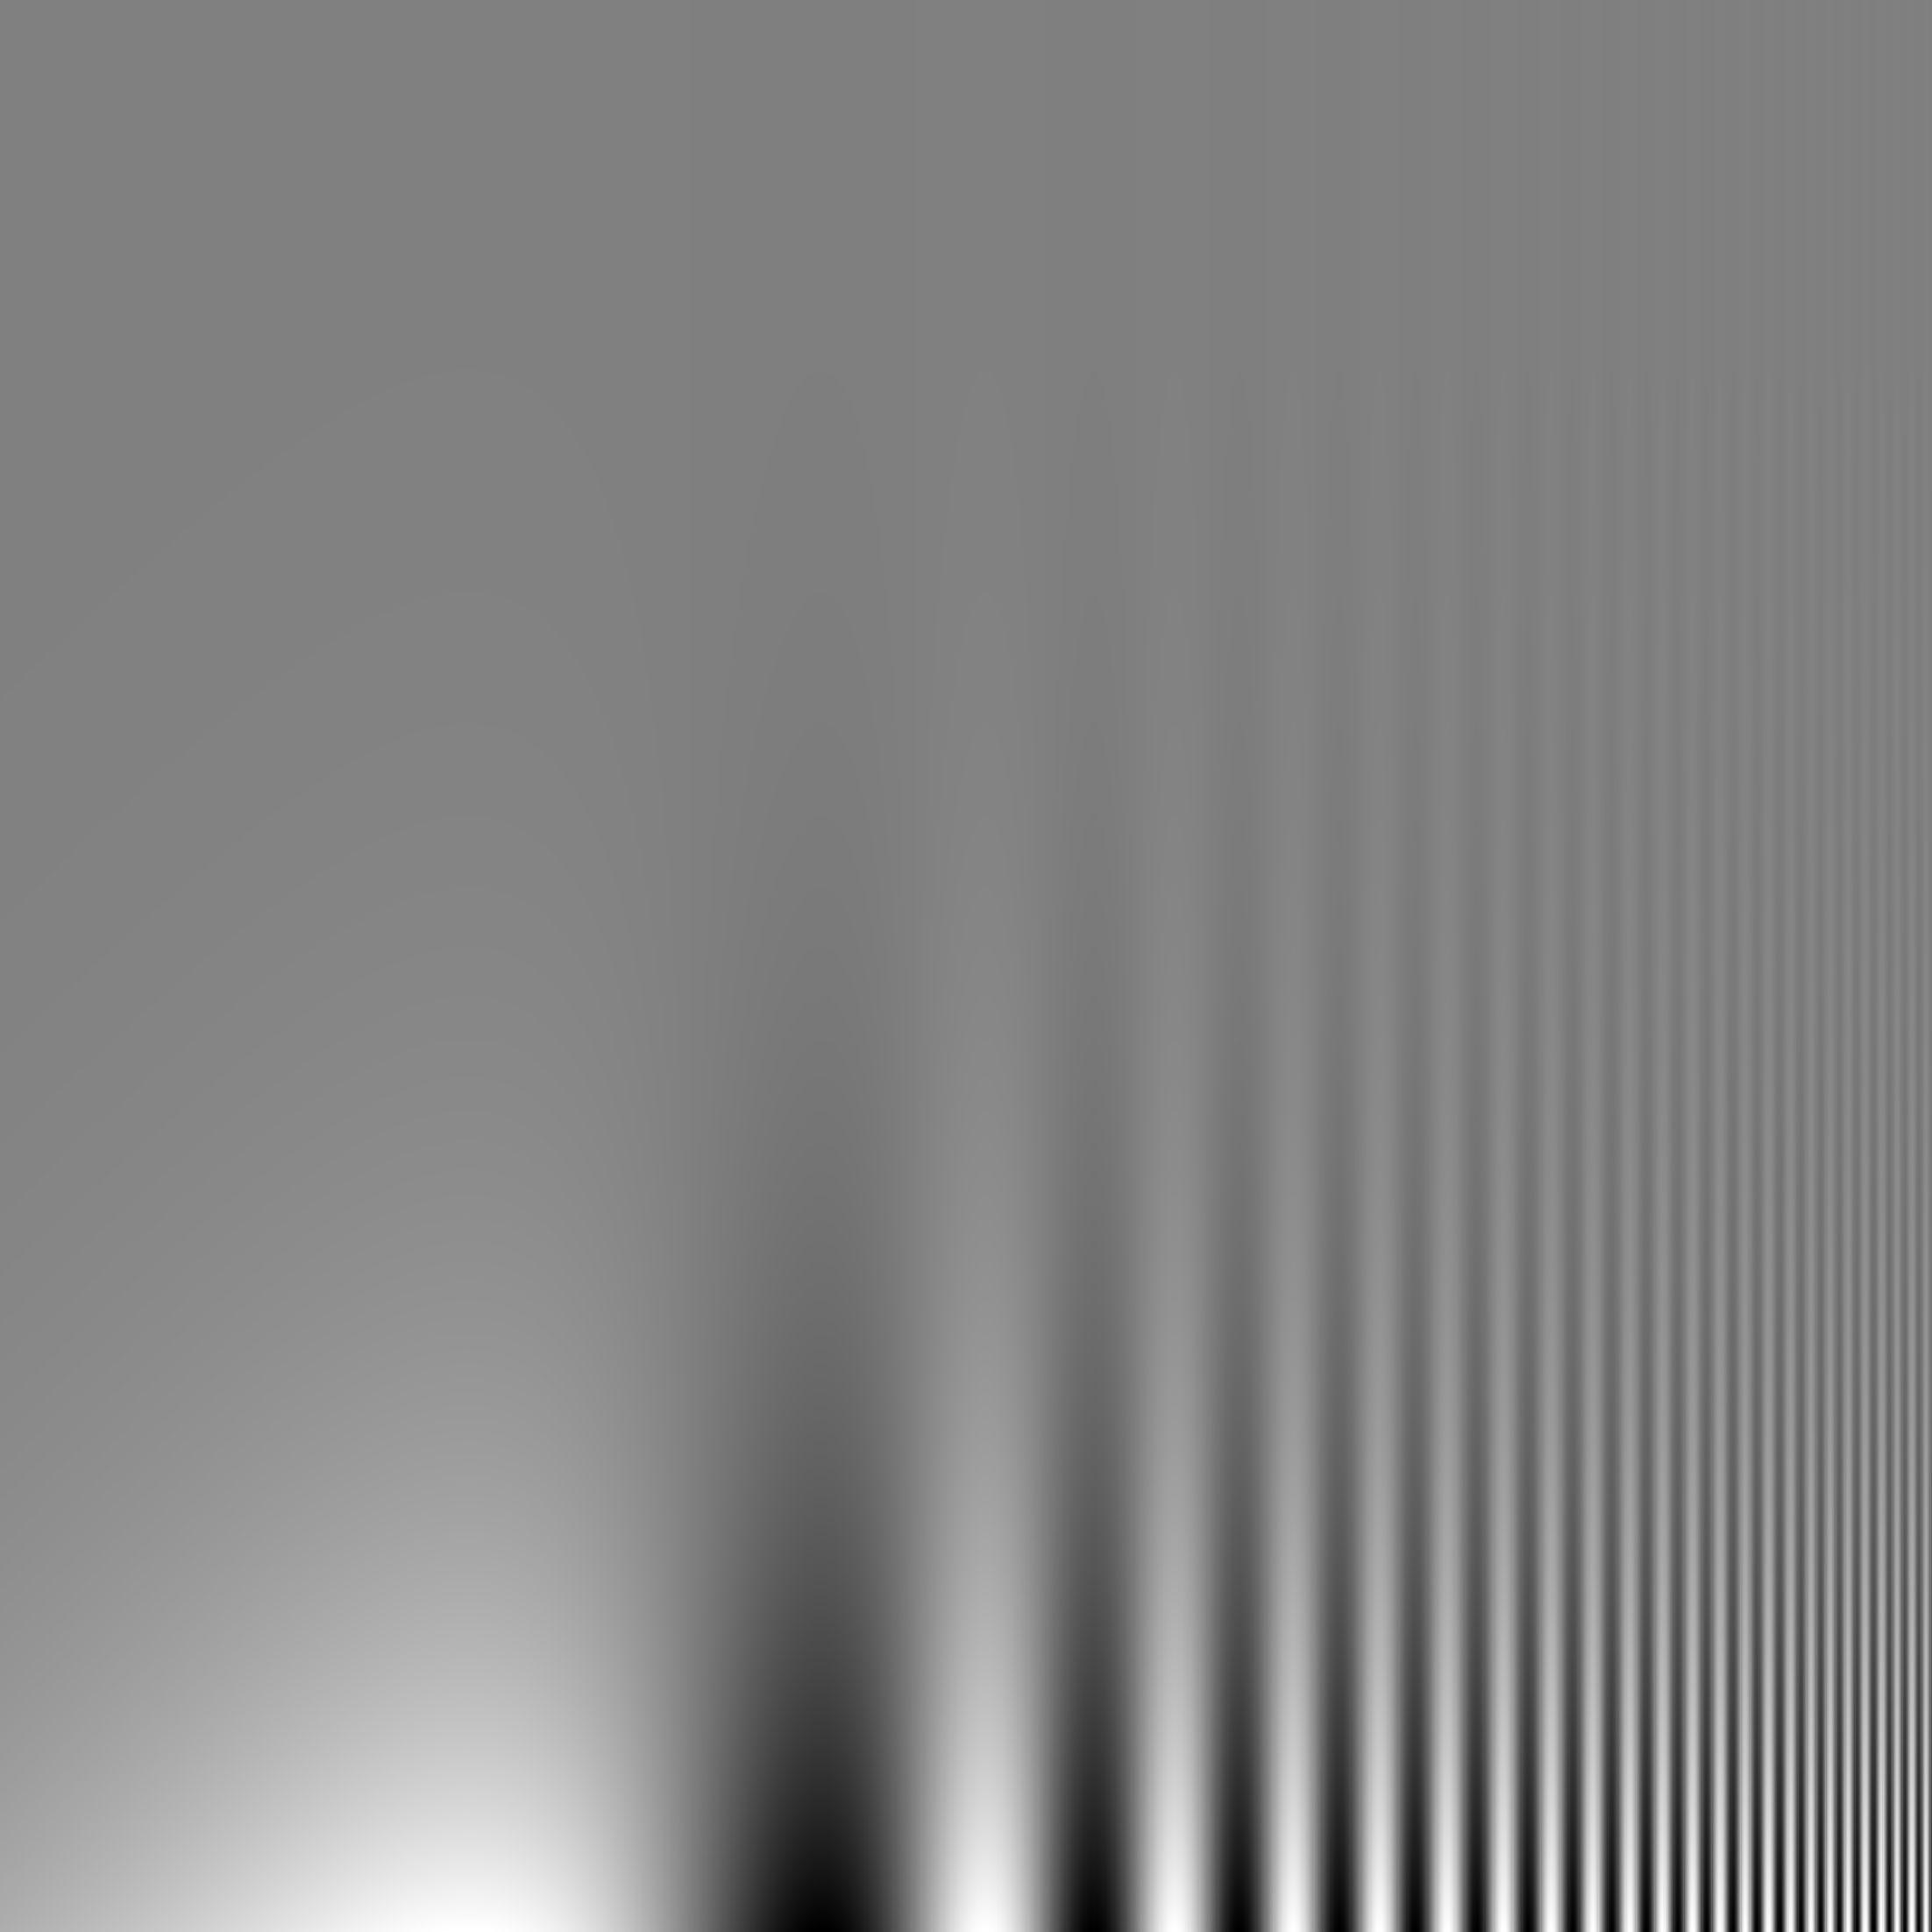
\includegraphics[width=0.235\linewidth]{chapter6/figures/scsf-gray}\qquad
	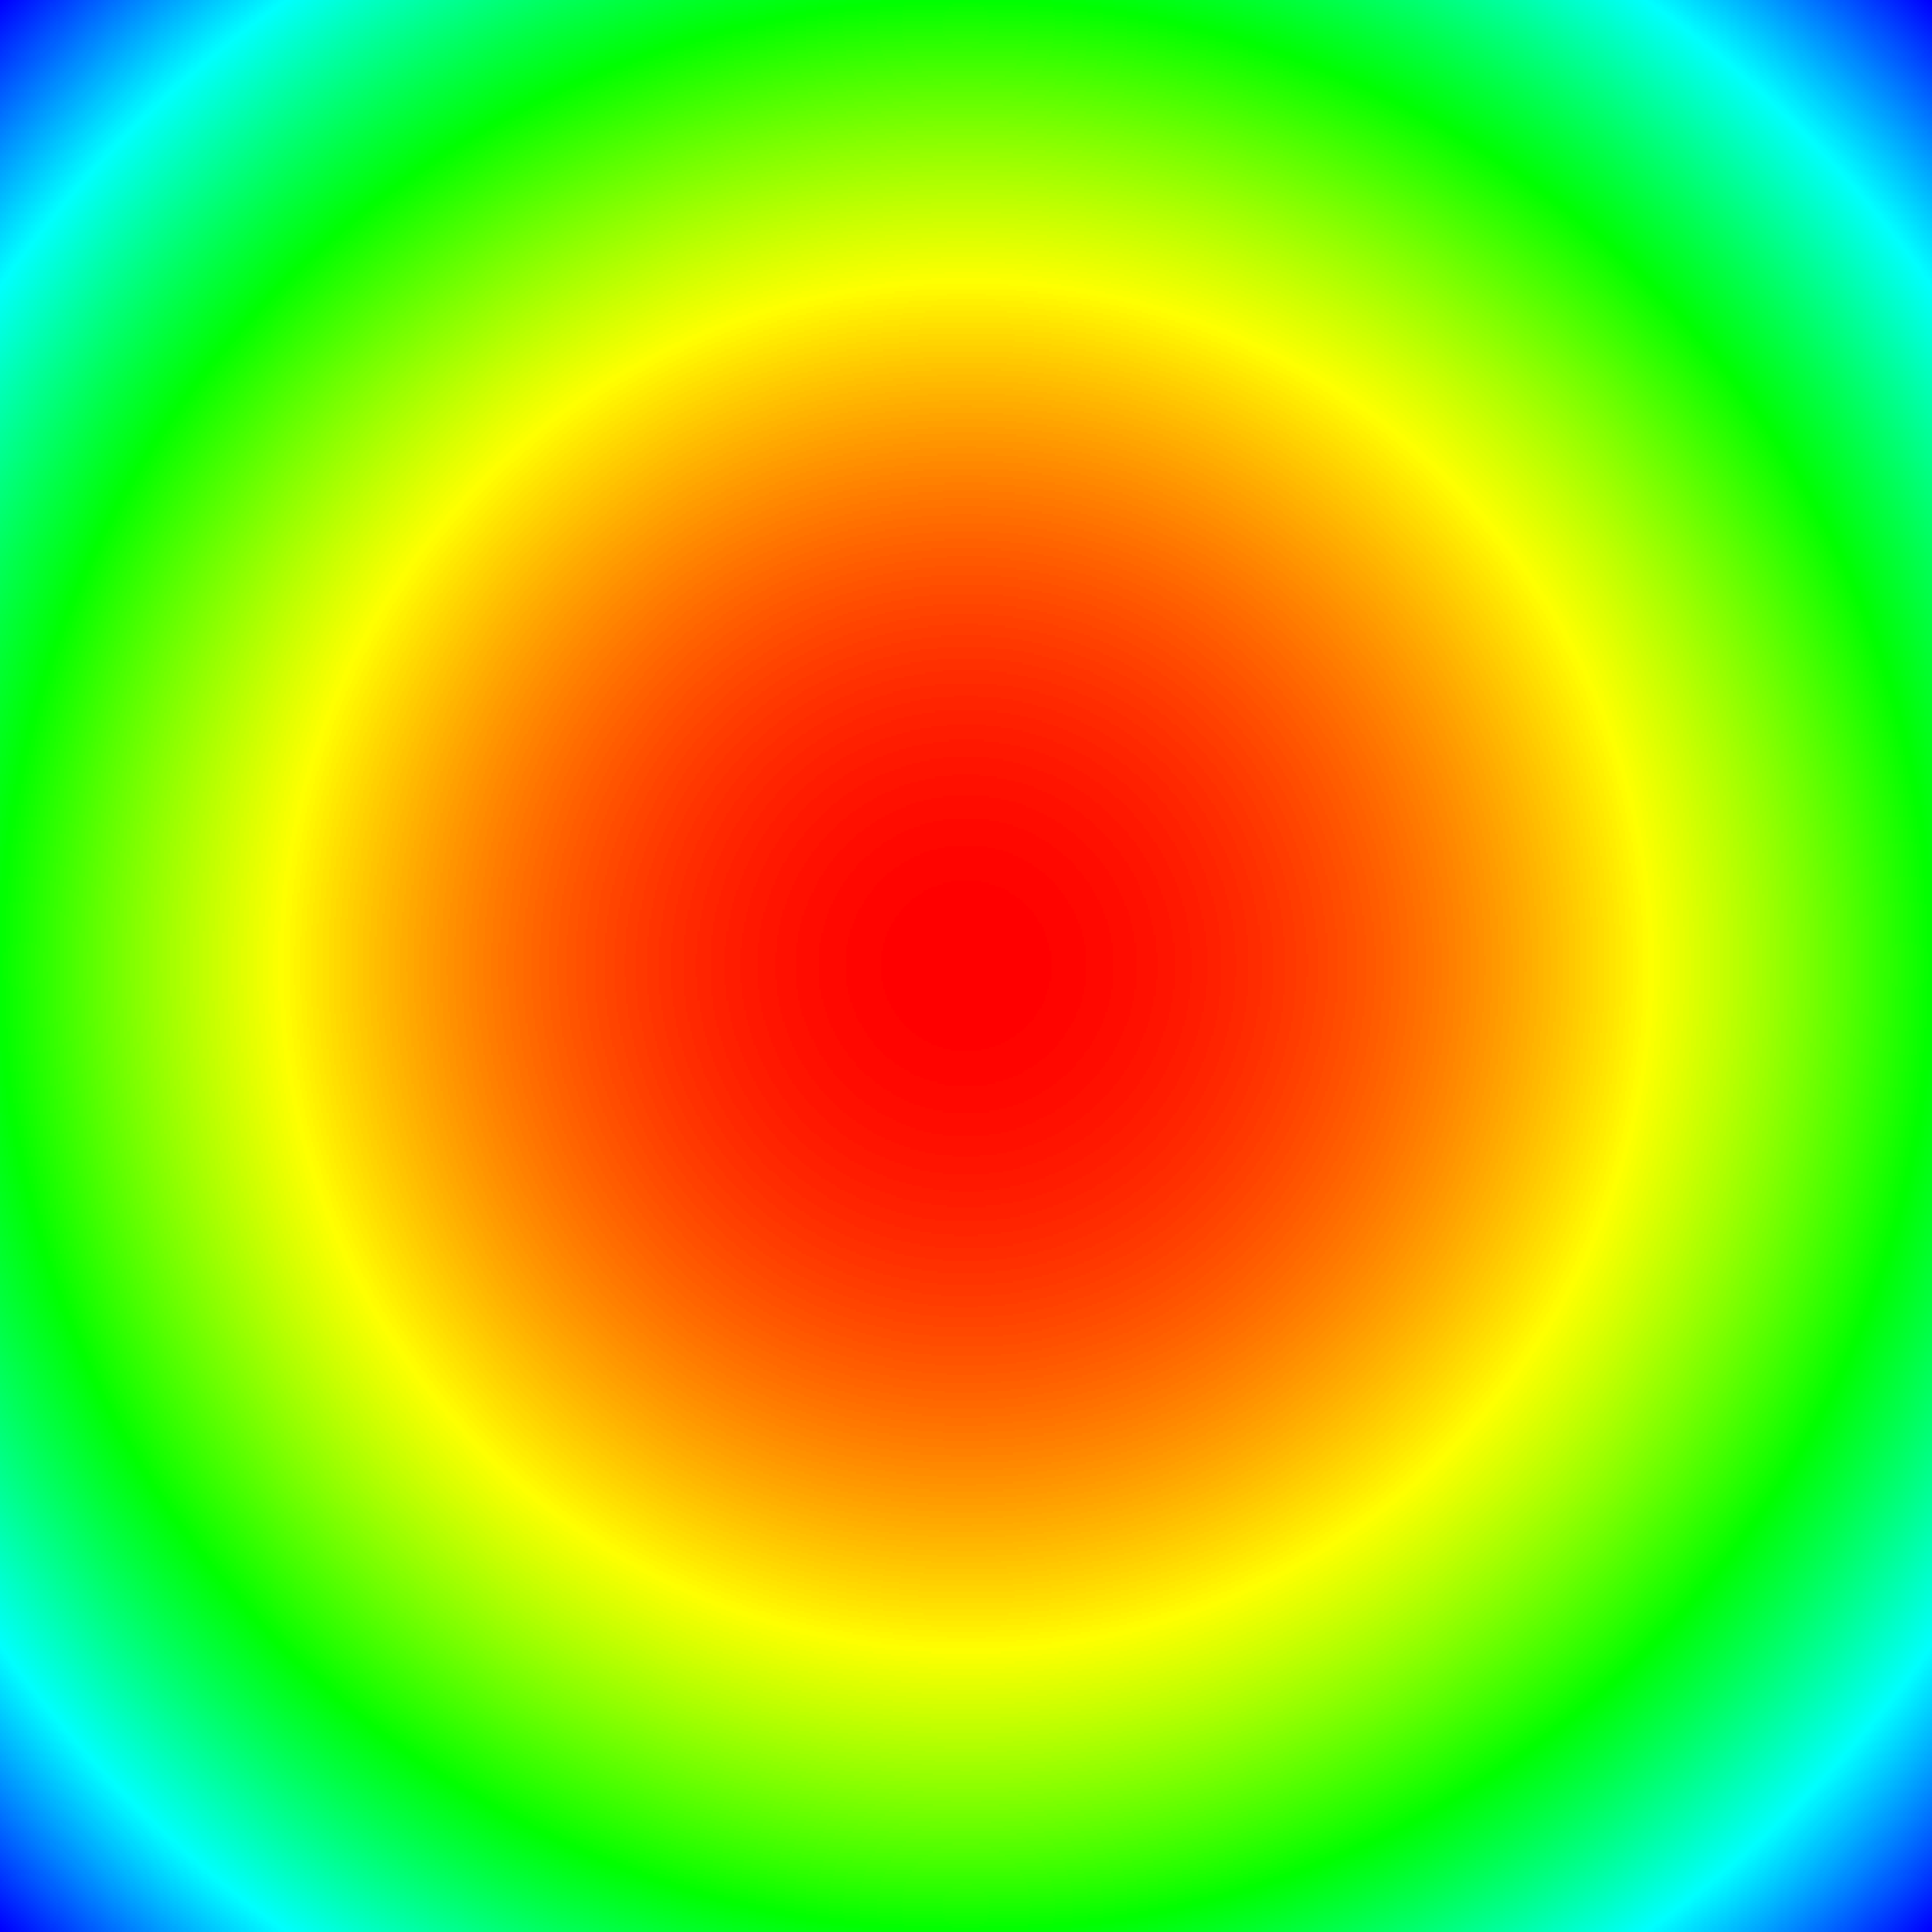
\includegraphics[width=0.235\linewidth]{chapter6/figures/hill-rainbow}
       
\includegraphics[width=0.235\linewidth]{chapter6/figures/hill-gray}\qquad
   \caption{Left: the images show the color mapping of the spatial contrast sensitivity function. Frequency increases from left to right whereas contrast increases from the top to the bottom. The isoluminance of the rainbow color map obfuscate low contrast regions and small details, which can be seen using gray scale. Right: changes in color in the rainbow color map may be perceived as features in the data. The ``boring'' scalar field $f(x,y) = x^2+y^2$ appears to have more features when rainbow color map is used than in the gray scale image.}
   \label{fig:rainbow}
 \end{figure}
%
Figure \ref{fig:rainbow} shows examples for each of these issues. 
%
The first issue is due to the lack of a \emph{natural sorting order}. Even though the rainbow color map 
is ordered from shorter to longer wavelength of light, users do not easily perceive it as such, which makes 
quantitative analysis more difficult\cite{Borland:2007:RCM:1251554.1251614}.  
%
In addition, the rainbow color map can \emph{obscure} data. The problem arises 
for data containing high spatial frequency. Isoluminant maps can obfuscate these frequencies 
because our visual system perceives them through changes in luminance. 
%
This is illustrated in the left images in Figure \ref{fig:rainbow}.
%
Note how details on the top half and left portions of the rainbow color mapped image  were ``removed'' by the choice of the color map.
%
Lastly, the rainbow color map can also add \emph{artifacts} to the visualization\cite{treinishshould}. 
The problem is that the gradient in color map creates the illusion of patterns where none exist. This 
is illustrated in the right image in Figure \ref{fig:rainbow}. In association with the lack of a natural sorting order, 
it becomes difficult to identify that patterns are not due to the underlying data but due to the color map. 
%
Although Figure \ref{fig:rainbow} shows simple synthetic examples, there have also been user studies and 
analysis showing that these problems are also present in the visualization of real world scenarios\cite{treinishshould}.
%
Despite its disadvantages, the rainbow color map is widely used in the sciences. In the study by Borkin 
\emph{et al.}\cite{305}, participants reported that they liked it because they are ``used to seeing'', that 
the saturated colors are ``easier to see'', and it is the ``most aesthetically pleasing''. 
%
Another possible reason  for its widespread use is that it is default in many popular simulation and 
visualization tools. Paraview is one of the tools that no longer uses the rainbow color map as the
default option since the publication of  Borland \emph{et al.}'s ``Rainbow Color Map (Still) Considered 
Harmful''\cite{paraview}. The author even suggest that a better name for it would be ``misleading color map''.
%


\begin{table}
\caption{Color maps in the AIAA journal} \label{table:aiaa_colormap}{}\centering
\begin{tabular}{lcccc}
				&  	Rainbow color map	 & Gray scale map & Other\\ \hline
	2010		&       68.63\%		   	 &        13.73\% & 17.64\%    		          \\
\gc	2011		& 		64.7\%		 	 &        15.69\%& 19.61\%      		     	  \\
	2012		&       79.03\% 	     &        8.65\% & 12.32\%        		      \\
\end{tabular}
\end{table}


In light of the many pitfalls of the rainbow color map, the visualization community has, in the past few 
years, been moving away from it. 
%
In 2005, $52\%$ of the scientific publication using a color map at the IEEE Visualization Conference 
had at least one occurrence of the rainbow color map\cite{Borland:2007:RCM:1251554.1251614}. 
This number has dropped to a single paper published at the {\em IEEE Transactions on Visualization and 
Computer Graphics} in 2011. Motivated by this experiment, we reviewed all publications from the 
{\em AIAA Journal} for the years of 2010, 2011, and 2012 that contained a color map and counted the number of papers that used the rainbow color map. Table \ref{table:aiaa_colormap} shows the obtained results. Note that we do not evaluate the potential problems caused by the rainbow color map. 
%
Nevertheless, we tried the methodology explained above for a flow simulation dataset. 
The left image in Figure \ref{fig:flowdata} shows the results of a flow simulation. Note how some regions are over emphasized (shown in red) while details are blurred (shown in green). The problems with the rainbow color map can be avoided by simply switching to another color map, such as the gray scale color map shown in the middle image in Figure \ref{fig:flowdata}. The image to the right shows the decolorized rainbow color map: although some details are easier to see, the result is still very different from the gray scale color map.

The visualization community has also investigated what should constitute a ``good'' color map. Research on the topic of color selection can be found in the work by Treinish \emph{et al.} \cite{treinishshould}, Moreland\cite{paraview}, Kindlmann \emph{et al.}\cite{GLK:facelum02}, and others\cite{macdonald1999using,Tominski:2008bt}. The AIAA community can benefit from a set of standard color maps suitable for visualization of typical simulation data such as pressure fields, angle fields, {\em etc.}

 \begin{figure}[tp]
 	\centering
       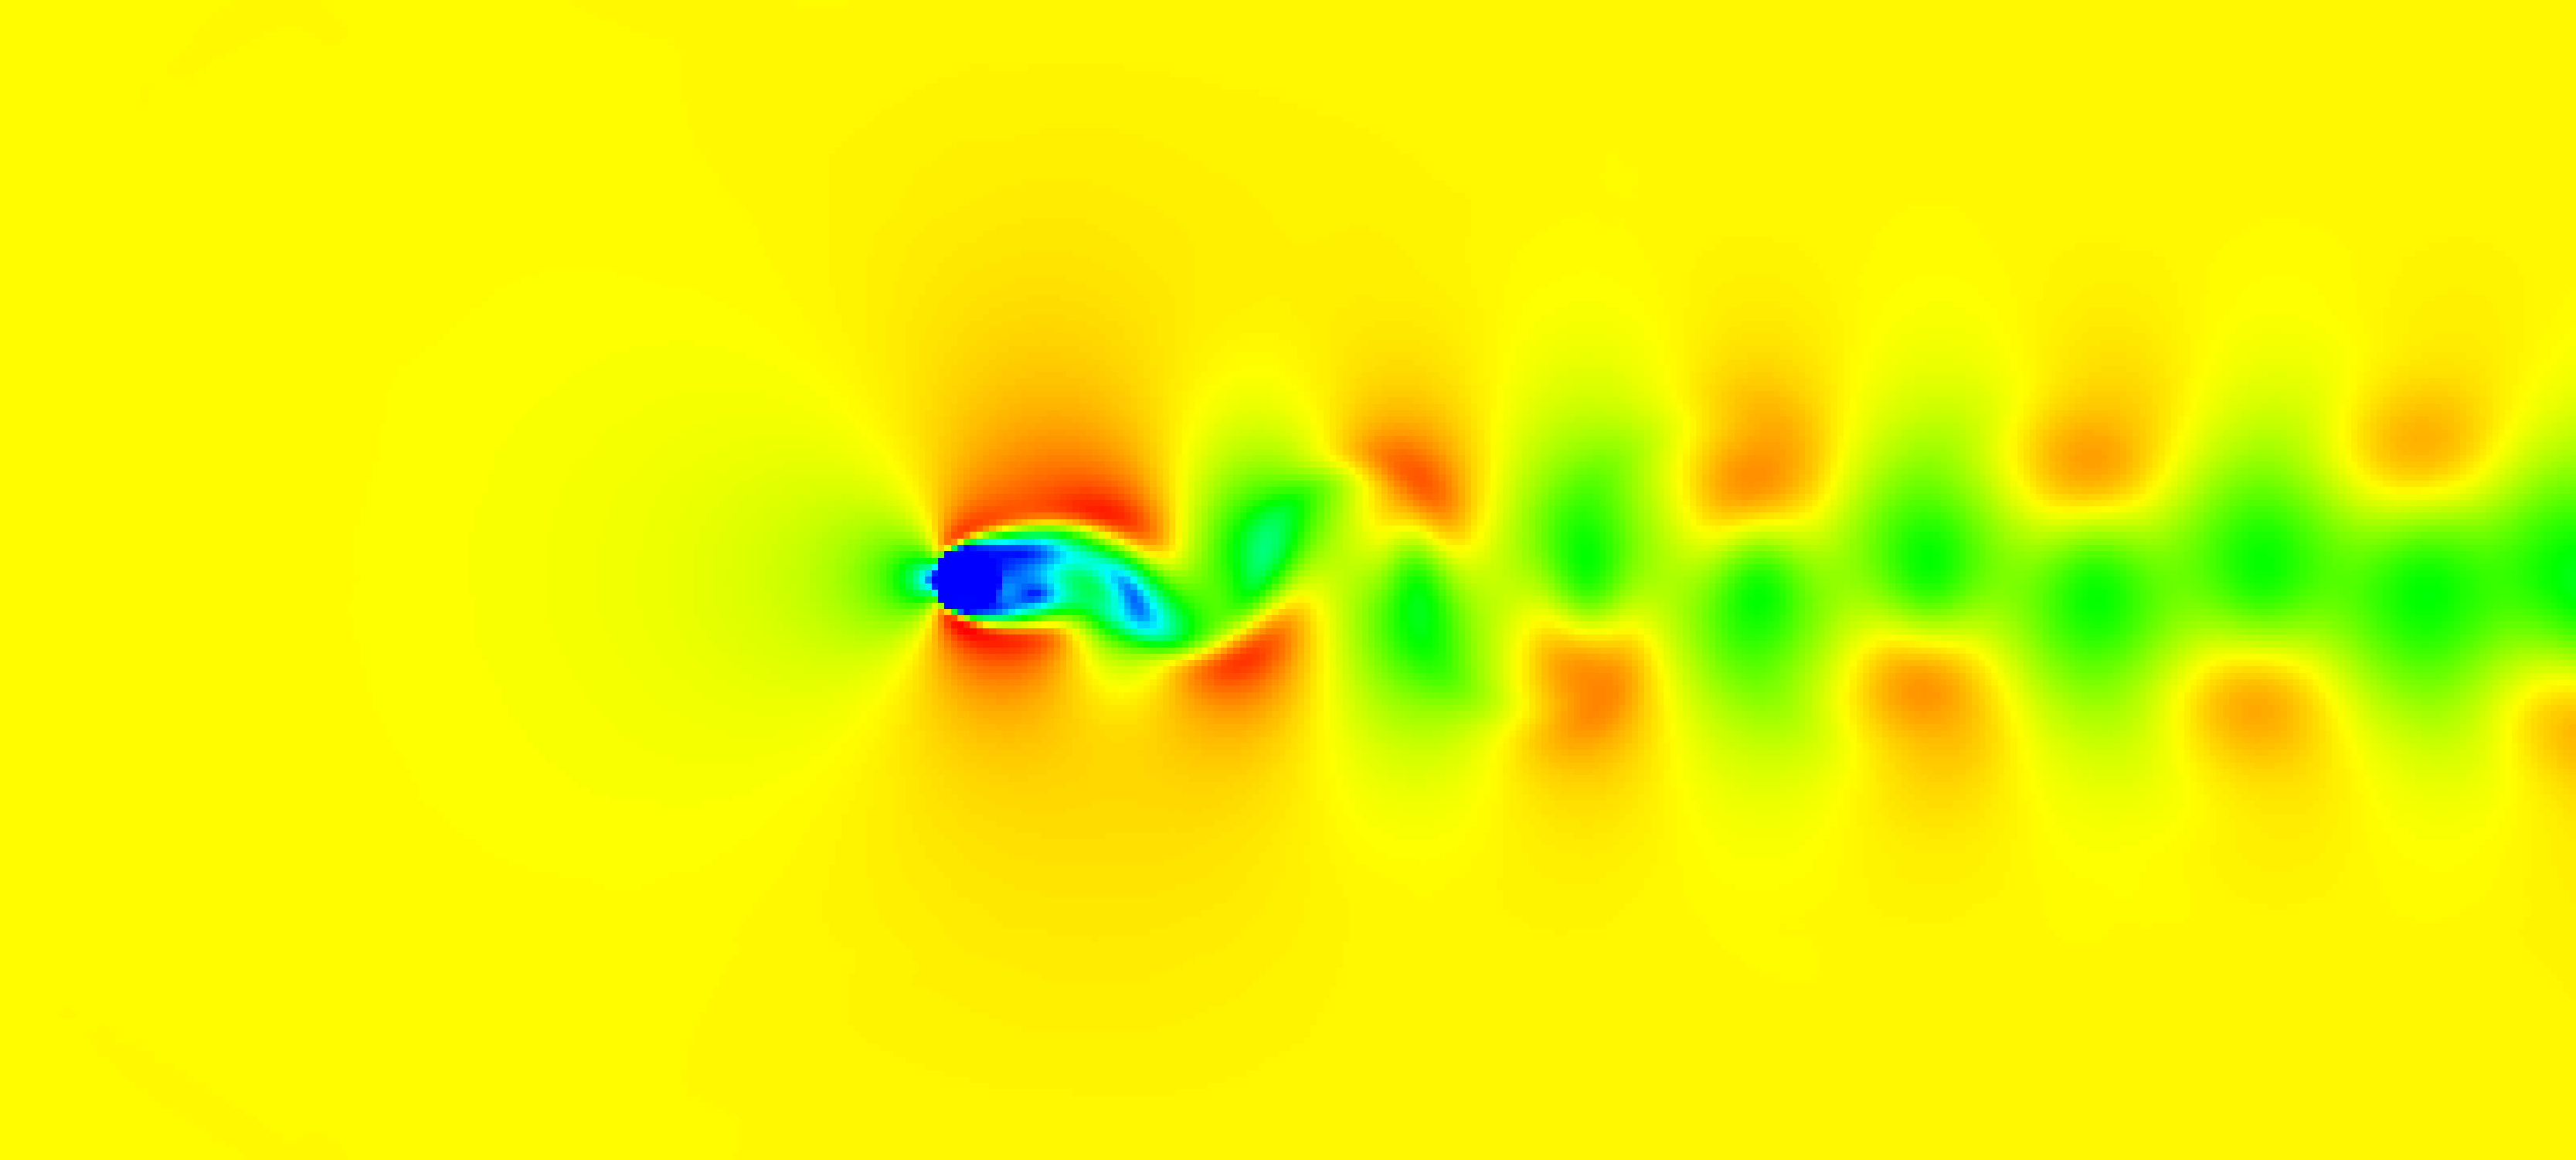
\includegraphics[width=0.325\linewidth]{chapter6/figures/vector_field_rainbow.png}
       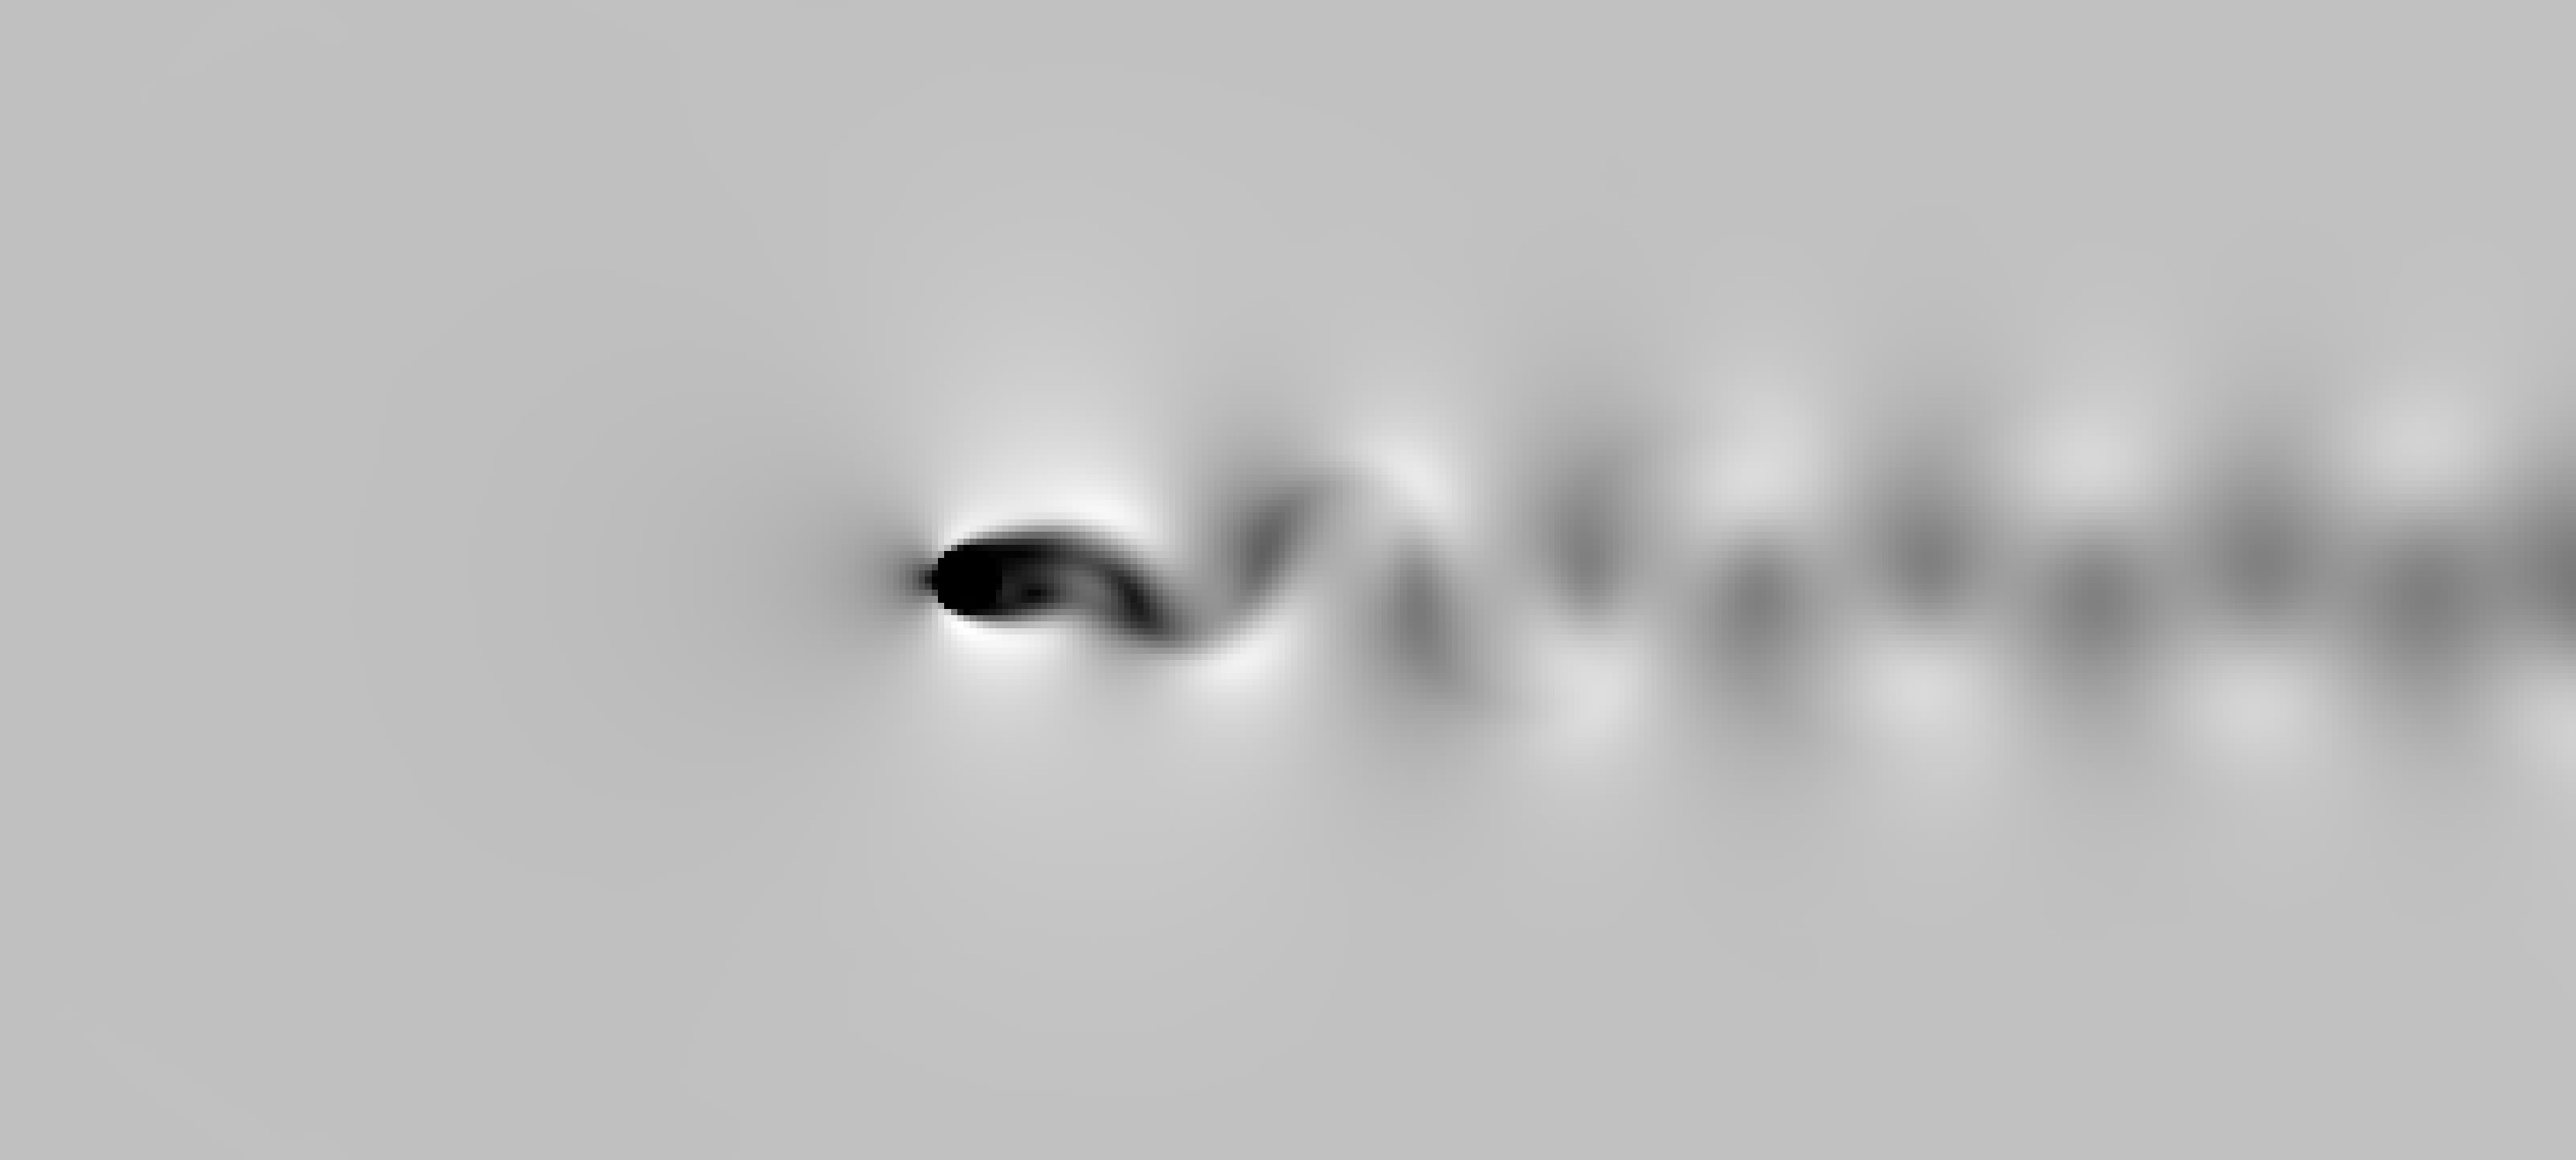
\includegraphics[width=0.325\linewidth]{chapter6/figures/vector_field_gray.png}
       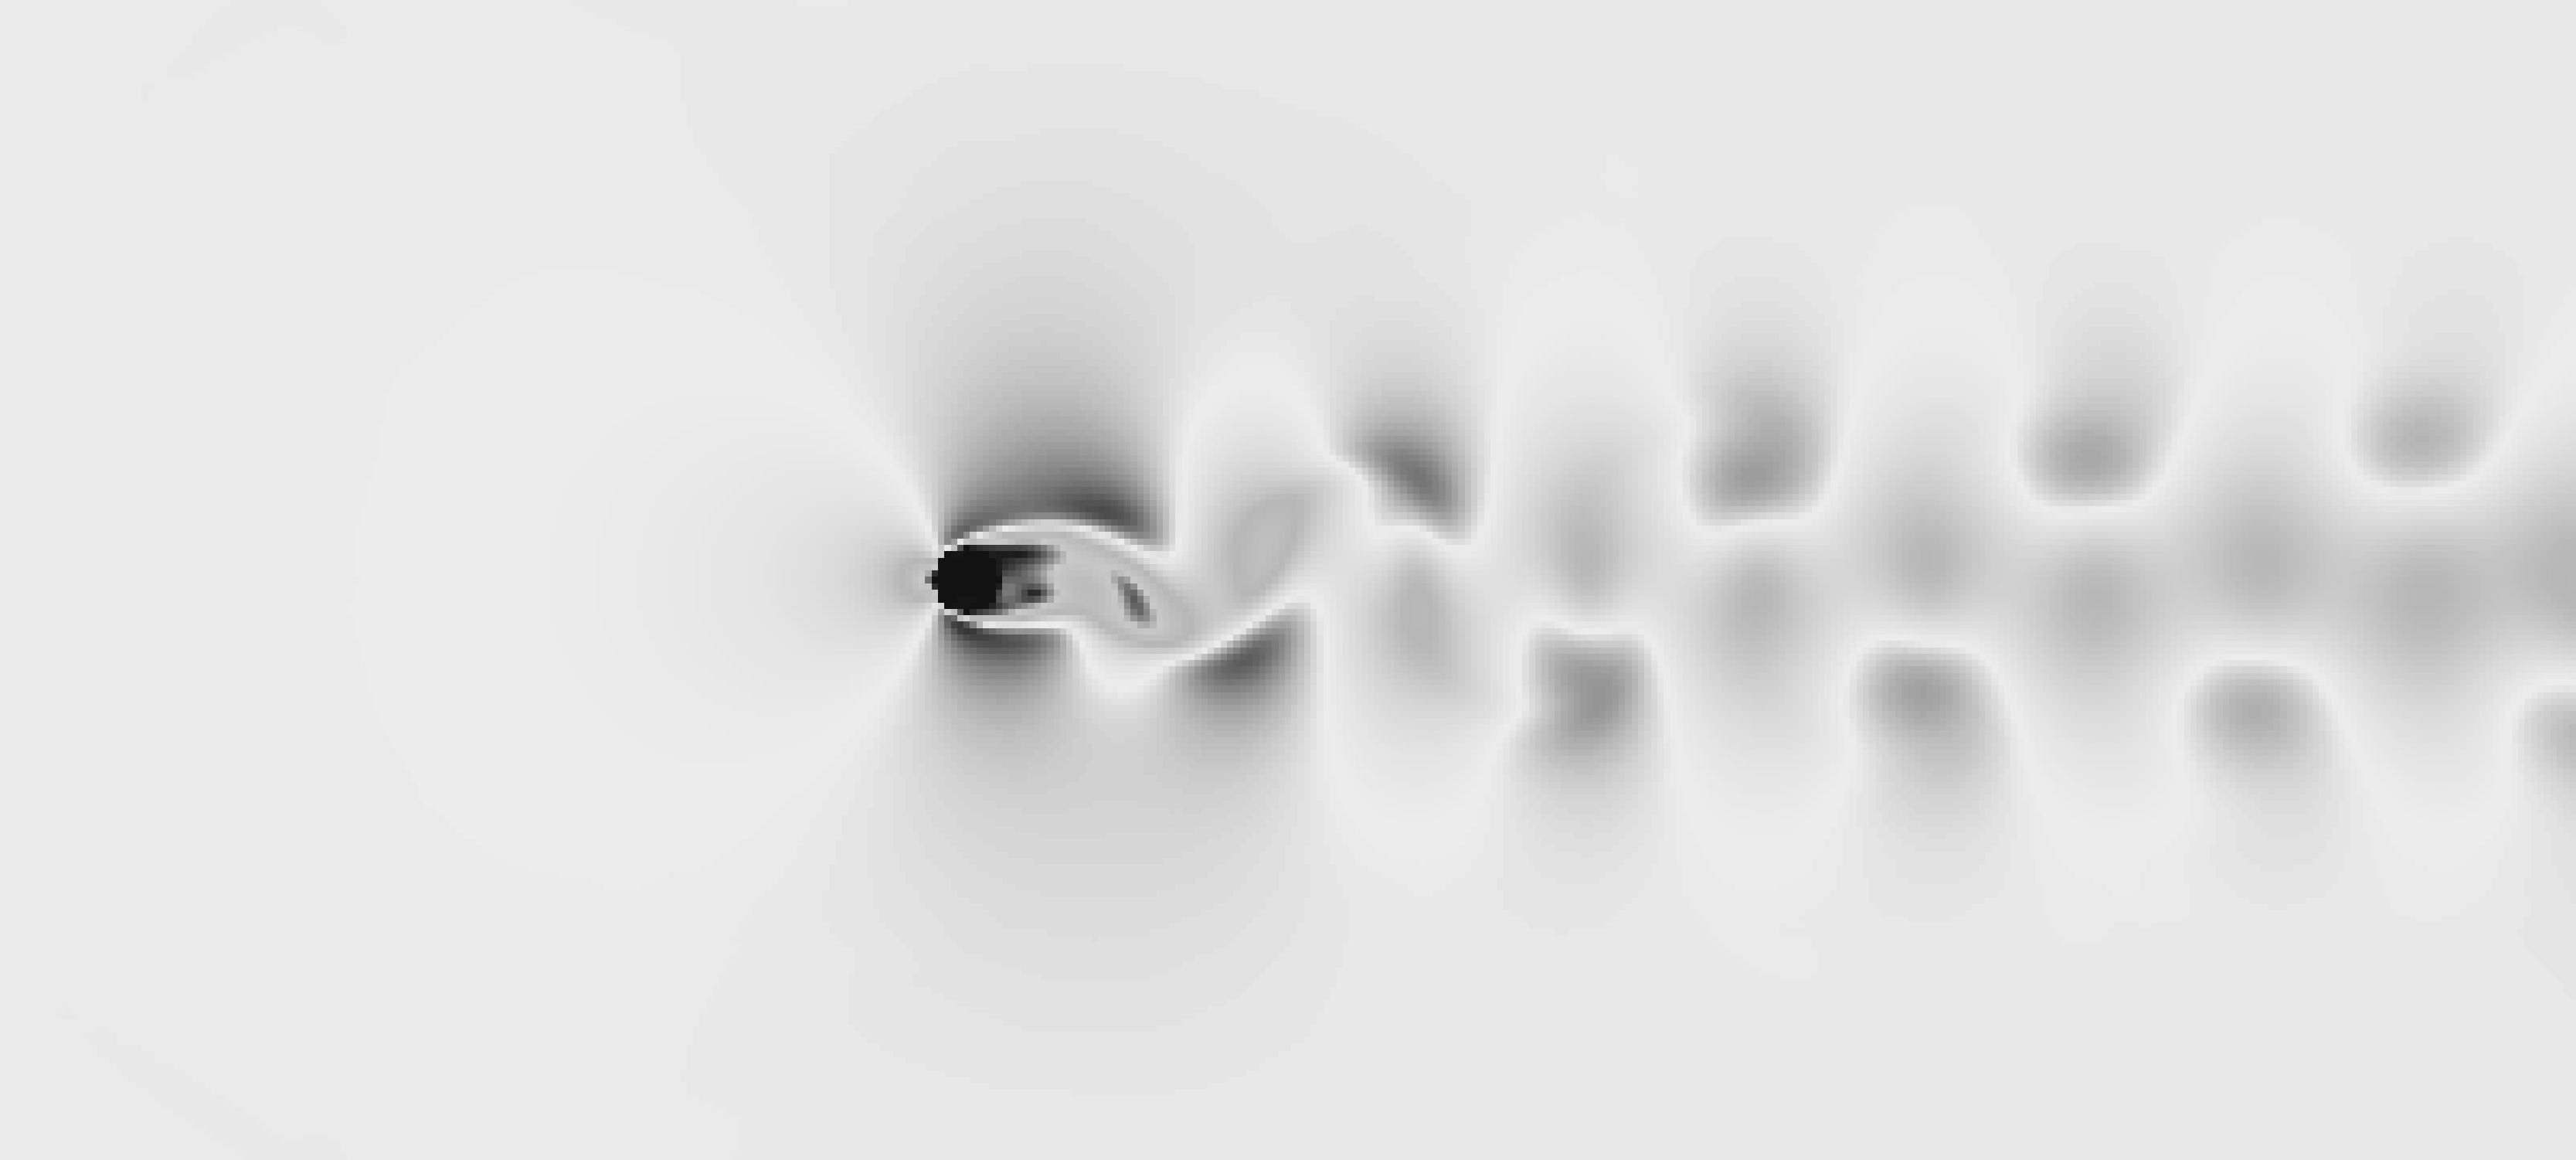
\includegraphics[width=0.325\linewidth]{chapter6/figures/vector_field_rainbow_then_gray.png}
   \caption{Velocity magnitude. Rainbow (left) and gray scale (middle) color maps were applied to a 2D flow simulation using a spectral element code for solving the incompressible Navier-Stokes Equations. Note how red regions on the rainbow color map are over emphasized while green regions ``blur'' details that are shown in the gray color map. The image on the right is the decolorized rainbow color map.}
   \label{fig:flowdata}
 \end{figure}

%- Reasons for the rainbow color map success.
%The works MacDonald\cite{macdonald1999using} and  Silva \emph{et al.}\cite{Silva2011320} 
%provide guidelines for the use of colors in computer graphics.

%Color is one of fundamental features in visualization. It can help visualization to label, to measure, 
%to represent or even to decorate the data sets or information. In these cases, color does no harm. 
%Paper ``Rainbow Color Map (Still) Considered Harmful'' by David Borland reiterates Rainbow Color 
%Map characteristics and still considers that Rainbow Color Map is poor choice. They mentioned that 
%a half of relevant papers in IEEE Visualization Conference proceedings still use rainbow color map. 
%This survey shows that researchers still use rainbow color map in visualization community. Also 
%ParaView, Matlab, VisADD, SCIRun and OpenDX use rainbow color map by default [1].

%However, when we took survey on rainbow color map in AIAA journals, AIAA papers used rainbow 
%color map but we could not find one AIAA paper discuss about this technique. They use rainbow 
%color map in 12.27\% of papers (33 papers over total 269 papers) in 2011 and 20.85\% (49 papers 
%over total 235) in 2012. And when we took survey on rainbow color map in IEEE transactions on 
%visualization and computer graphics, they still published one paper in 2011 and one paper in 2012. 
%We can see that they did not use rainbow color map much like before 2007. A paper of IEEE 
%transaction on visualization and computer graphics do research on rainbow color map but also 
%confirm that rainbow color map can significantly reduce a person�s accuracy and efficiency. These 
%gives us some questions, why rainbow color is used very often in non-technique papers, do they 
%aware about their limitations?, should AIAA papers use rainbow color map or Visualization 
%community should change to use other color map techniques than rainbow color map technique? 
%and what color map technique that we should use instead of rainbow color map?

%Firstly, rainbow color map has some advantages that made researchers in visualization community 
%used that and make it by default in almost visualization toolkits. It makes the visualization 
%applications more pretty and attracted users� attentions but do not focus on actual information. 
%Rainbow color map has many problems and it was confirmed by some quantitative studies [2,3] and 
%they propose the better color map techniques for visualization such as isoluminant maps are 
%suitable. Rainbow color map confuse the users, obscuring data and misleading interpretation [1].  
%Because rainbow color map is orders from shorter to longer wavelength of light but it is not 
%perceptually ordered so if we use it to represent the ordered data, it will make users confused.

%Rainbow color map still is default for many visualization toolkits while researches tend to use less 
%rainbow color map in visualization community and very rarely in society. Should these toolkits 
%change their default of rainbow color to make it more efficient in programming for programmers?

%From the above analysis, we recommend that AIAA papers should not use rainbow color map that 
%often and Visualization community should do research to propose the best color map to replace 
%rainbow color map and visualization toolkits should change their default of rainbow color map to 
%more efficient color map technique.

%Then, we come up with important question of what color map techniques are better than rainbow 
%color map and which technique is the best should we use by default for color map? It is difficult 
%question because the best color map technique depends on users� tasks and context of applications.

%Other color map techniques such as Grayscale, Black-Body Radiation and isoluminant color map 
%[4] can be used instead of rainbow color maps to represent data more efficiently and more 
%accurately.

%[1] David Borland and RussellM., Rainbow Color Map (Still) Considered Harmful, Visualization 
%Viewpoints, March /April 2007.

%[2] G. Kindlmann, E. Reinhard, and S. Creem. Face-based luminance matching for perceptual 
%colormap generation. �, 2002.

%[3] B. Rogowitz and A. Kalvin. The which blair project: A quick visual method for evaluating 
%perceptual color maps. Proceedings of the conference on Visualization�01, pages 183�190, 2001.

%[4] http://paraview.org/ParaView3/index.php/Default_Color_Map

% write about visualization in common of vis community and what is vis perspective of AIAA


\subsection{Evaluation \& user studies}

In recent years, the Visualization community has seen a substantial increase in the number of papers dealing with evaluation of visualization techniques published within {\em IEEE TVCG}.  Figure \ref{fig:tvcg} shows the number of such papers published per year within the {\em IEEE TVCG} journal. The data was obtained by searching the {\em TVCG} website for the keywords ``evaluation'', ``user study'', ``design study'', and ``case study'' in articles published in the period between 2002 and 2012. We then read the abstracts to make sure the papers were indeed relevant. From this corpora, $96\%$ of the aforementioned articles were user studies.

%We searched IEEE Transactions on Visualization and Computer Graphics (TVCG) from 2002 to 2012 for papers with some current visualization trends such as design study, case study, user study, uncertainty visualization, verification, validation and evaluation. Table 1 shows the statistics and trends from 2002 to 2012 IEEE TVCG papers present design study, case study, user study, uncertainty visualization, verification, validation and evaluation.
%Figure 2 also shows the trends of these popular techniques in visualization community from 2002 to 2012. We can see that evaluation technique is more popular in visualization community than 6 other visualization techniques and it grow much in 2011. User study technique is increased much more in 2011 and 2012.

%\begin{table}
%\caption{Statistics from 2002 to 2012 IEEE TVCG papers present design study, case study, user study, uncertainty visualization, verification, validation and evaluation} \label{table:tvcg_search}{}\centering
%\begin{tabular}{lcccccccccccccc}
%No	& Keywords	&  2002&	2003&	2004	&2005&	2006	&2007&	2008&	2009	&2010	&2011&	2012 \\ \hline
%1&	design study	&	0& 0	&	0	&0	&1&	0	&3	&3&	1	&2&	0 \\
%2&	case study		&	0&	0	&	0	&0	&5	&3	&3	&7	&4	&8	&4 \\
%3&	user study		&	0&	1	&1	&2	&7	&6	&4	&5	&9	&14	&18 \\
%4&	uncertainty		&	0&	0	&1	&1	&1	&4	&3	&4	&8	&6	&2 \\
%5&	verification		&	0&	0	&0	&0	&0	&2	&0	&1	&0	&1	&3 \\
%6&	validation		&	0&0	&0	&0	&1	&1	&2	&3	&0	&2	&3 \\
%7&	evaluation		&	4&0	&4	&9	&18	&16	&21	&24	&22	&28	&23 \\
%\end{tabular}
%\end{table}

%\begin{table}
%\caption{Table summary}{lcccccccccccccc}
%No	& Keywords	&  2002&	2003&	2004	&2005&	2006	&2007&	2008&	2009	&2010	&2011&	2012 \\ \hline
%1&	design study	&	0& 0	&	0	&0	&1&	0	&3	&3&	1	&2&	0 \\
%2&	case study		&	0&	0	&	0	&0	&5	&3	&3	&7	&4	&8	&4 \\
%3&	user study		&	0&	1	&1	&2	&7	&6	&4	&5	&9	&14	&18 \\
%4&	uncertainty		&	0&	0	&1	&1	&1	&4	&3	&4	&8	&6	&2 \\
%5&	verification		&	0&	0	&0	&0	&0	&2	&0	&1	&0	&1	&3 \\
%6&	validation		&	0&0	&0	&0	&1	&1	&2	&3	&0	&2	&3 \\
%7&	evaluation		&	4&0	&4	&9	&18	&16	&21	&24	&22	&28	&23 \\
%\end{tabular}
%\end{table}

\begin{wrapfigure}{r}{0.4\textwidth}
  \begin{center}
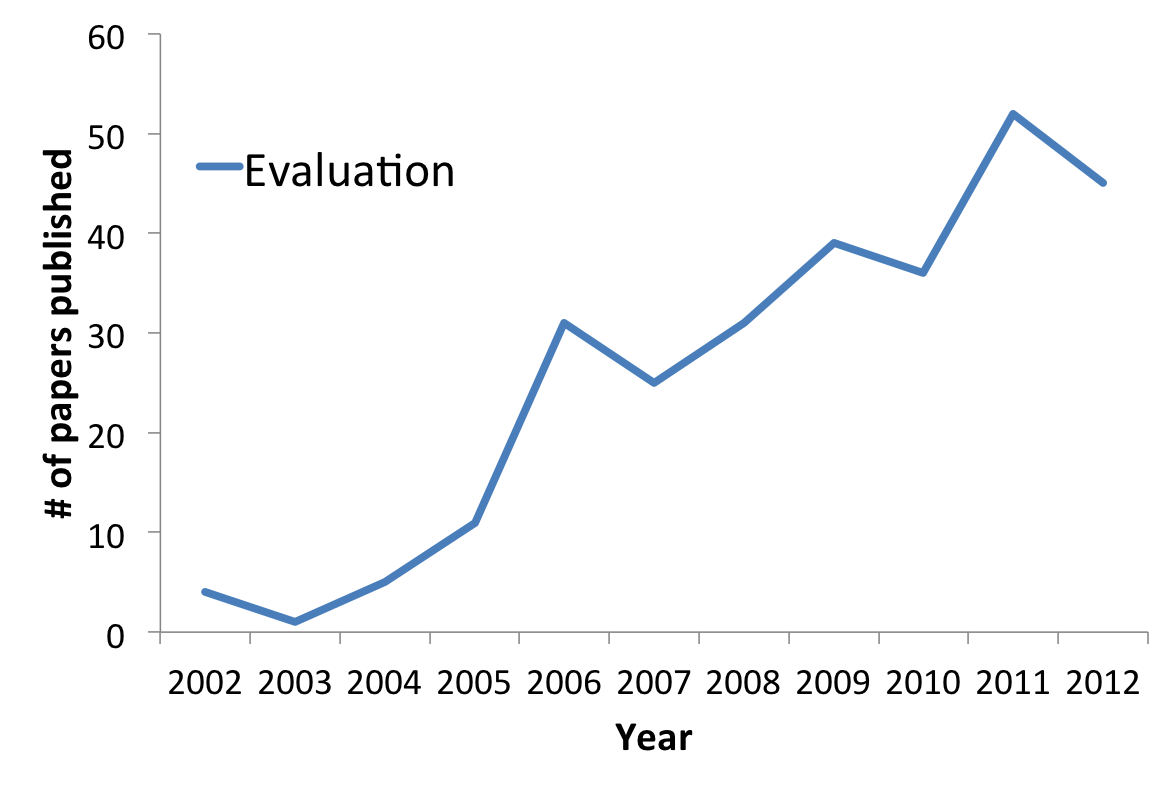
\includegraphics[width=0.38\textwidth]{chapter6/figures/evaluation_tvcg.png}
  \end{center}
  \caption{\label{fig:tvcg}Evolution of the number of papers published on the topic of evaluation at TVCG.}
\end{wrapfigure}
 
%With user study technique in 2011 and 2012, $94\%$ papers conducted their own user study with number of participant is less than 70. Only $6\%$ papers used the previous works to get the results of user study. 
%
%[This goes to the opportunities section] We also reviewed all user study papers of IEEE TVCG from 2008 to 2012 and found that almost papers did not cite papers from non-technique community such as AIAA community. Some papers cite papers from non-technique community less than $20\%$ of total reference papers. 
% will write more this part

As a representative example, we focus on a user study by Laidlaw \emph{et al.}\cite{Laidlaw:2005:CVF:1032290.1032538} comparing techniques for the visualization of steady 2D vector fields.
The authors recruited five experts and 12 non-experts users to evaluate the efficacy of each of the six techniques displayed in Figure \ref{fig:user_study}. The evaluation was measured by the user performance during the execution of several tasks of three types: critical point detection; critical points classification; and simulation of particle advection. The first two tasks are standard whereas the third task is motivated by the fact that often experts were interested in the global flow direction. The three tasks were chosen based on the authors interaction with fluid mechanics researchers. 
The authors built a collection of 500 vector fields for evaluation of the tasks. Among the results, they cite no significant difference between experts and non-experts regarding accuracy in the tasks or the response times. More interestingly, performance when using the standard method of arrows on a regular grid (GRID in Figure \ref{fig:user_study}) falls below average for multiples tasks involving critical points location, classification and advection (which means that users required more time to complete the task and committed more errors). On the other end of the spectrum, user performance when using GSTR consistently scored above average. Another similar study compare the user performance when using line and tube integral curves (with monoscopic and stereoscopic viewing) for 3D vector field data\cite{Forsberg:2009:CVF:1638611.1639226}. User study can be a powerful tool for helping users choose the best tool for their needs and the visualization community has been working on evaluating and testing techniques as they become more widespread.

 \begin{figure}[tp]
 	\centering
       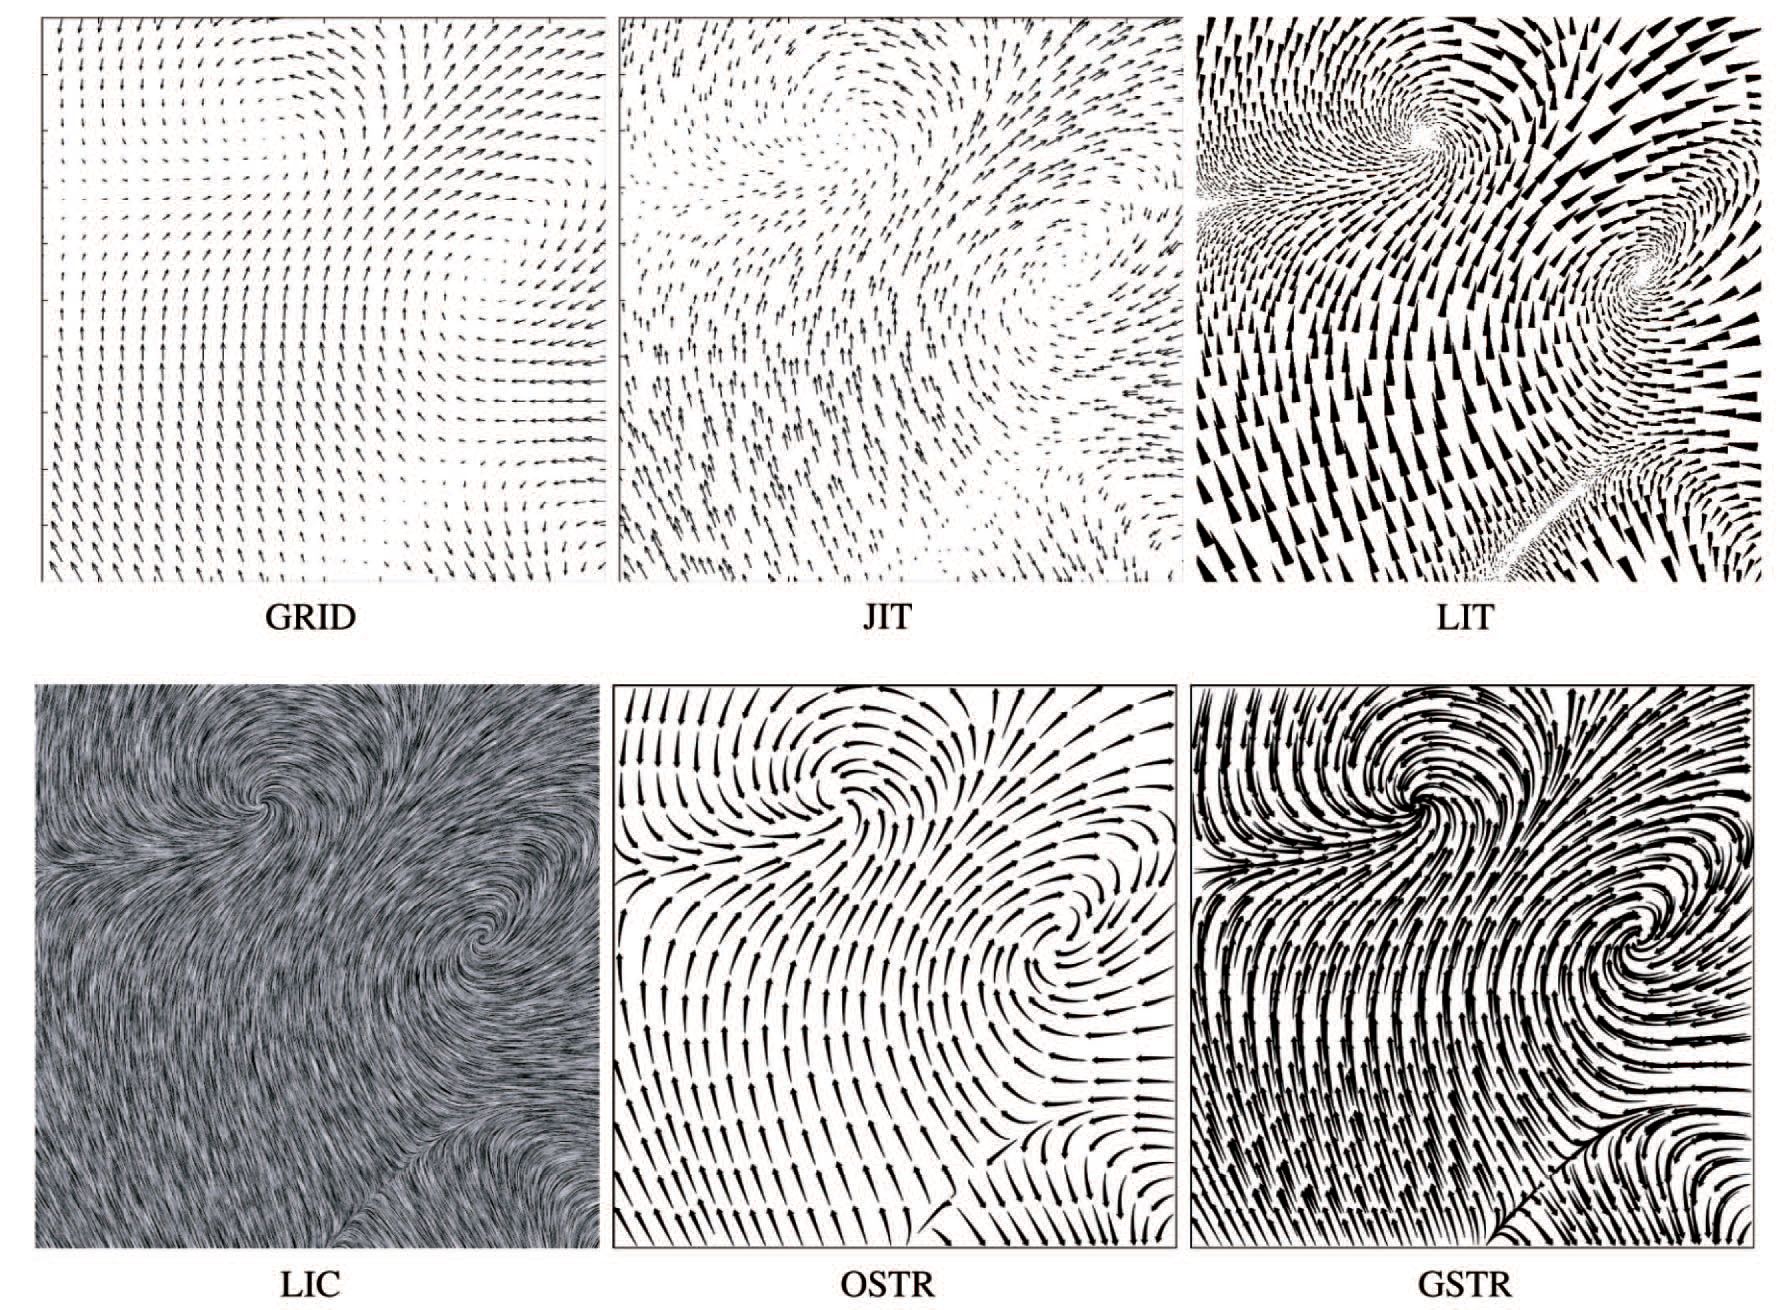
\includegraphics[width=0.835\linewidth]{chapter6/figures/ust_kirby}
   \caption{Comparing visualization methods for steady 2D vector fields. Top: standard arrow visualization, jittered arrow, icons using concepts borrowed from oil painting, respectively. Bottom: line-integral convolution, image-guided streamlines, streamlines seeded in a regular grid, respectively.}
   \label{fig:user_study}
 \end{figure}
 

%There are some methods of user study researchers can use such as list of questions and answers for users or define tasks and number of users to test their methods or systems to get the answers. For example, \cite{Comparing 2D Vector Field Visualization Methods: A User Study} published one paper in TVCG of comparing 2D vector field visualization methods by user study. They generated 500 3D vector field data sets from images and defined tasks to compare 6 visualization methods such as GRID, JIT, LIT, LIC, OSTR, and GSTR. The tasks is representative of interactions that users perform with different visualization methods. The authors also interviewed fluid mechanics researches to identify good representative tasks. The users are 5 experts and 12 non-experts. From this user study, they can figure out which technique perform the best. These paper's results will be good recommendation visualization techniques that AIAA community and other communities should use. 

% number of user study
%[We need to talk about this] There is a question on how many users should use in user study? In 50 papers of user study in TVCG from 2008 to 2012, there are only 2 papers use more than 70 users, otherwise use less than 70 users such as  \cite{Evaluating Sketchiness as a Visual Variable for the Depiction of Qualitative Uncertainty} paper user 1136 participants. $93\%$ of these papers conducted their own user study and $7\%$ papers user previous works. These user study papers mentioned less than 7 techniques. 

% question
%[We need to talk about this] AIAA community will be good users for Visualization community's user study. AIAA community can give us list of questions on visualization techniques that Visualization community proposed. They also can feedback with the best answers after they do experiments or interact with visualization techniques or systems. By this way, both communities can support each others and make visualization communities' proposals useful.


%%%%%%%%%%%%%%%%%%%%%%%%%%%%%%%%%%%%%%%%%%%%%%%%%%%%%%%%%%%%%%%%%%%%
\section{Uncertainty and Verification}
\label{sec:verif}

Uncertainty visualization  and  visualization verification  are two important topics in the pursuit for reliable visualizations. 
The AIAA community is  familiar with both topics. In this work, however, we present some of the recent advancements in this area from the point of view of the Visualization community. The goal is to increase the user confidence in the results of the visualization by answering questions such as: how can one visualize the inherent error sources in the visualization? or, how can one increase her/his confidence that an implementation of a visualization algorithm  does what was intended? In the following sections we present some of the recent developments in uncertainty visualization and the verification of isosurface extraction techniques.

%Amidst the several available techniques, many questions are asked by the diligent practitioner: how techniques compare to each other? What are the best techniques available for a given scenario? How can we measure and visualize the different error sources? How can one make sure that the results of the visualization are actually showing what it was intended? The AIAA community has already a tradition of carefully handling some of these topics in their domain. Nevertheless, the visualization is often considered as a post-processing and many times experts and practitioners are not fully aware of the ideas used behind the scenes along with its limitations and guarantees. Recently, the visualization community has undertaken many of these tasks in order to improve reliability of visualization procedures. In this section, we briefly review some of the advances in the reliability of visualization techniques. 

% will insert figures and more details of paper [1]

\begin{figure}[ht]
\centering

\includegraphics[width=0.9\linewidth]{chapter6/figures/curve.png}
\caption{The four uncertainty visualization methods used by Sanyal \emph{et al.}\cite{Sanyal:2009:USC:1638611.1639227} in their user study. From left to right: glyphs size, glyphs color mapping, surface color mapping, and error bars.}
\label{fig:uncertainty_user_study}
\end{figure}

%\begin{figure}[ht]
%\centering
%\includegraphics[width=0.3\linewidth]{chapter6/figures/p1.jpg}
%\includegraphics[width=0.3\linewidth]{chapter6/figures/p2.jpg}
%\includegraphics[width=0.3\linewidth]{chapter6/figures/p3.jpg}
%\includegraphics[width=0.3\linewidth]{chapter6/figures/p4.jpg}
%\includegraphics[width=0.3\linewidth]{chapter6/figures/p6.jpg}
%\caption{Uncertainty Visualization 3D}
%\label{fig:uncertain_user_study}
%\end{figure}

\subsection{Uncertainty visualization}

In the course of scientific inquiry, uncertainty is the norm. The visualization community has recently turned its attention to uncertain data, and is trying to solve problems on how to best compute and convey uncertainty information. Since 2010, around 30 papers were published at {\em TVCG} on the topic, with application on information visualization and scientific visualization. So far, the community has seen several different representation for uncertainty, varying from traditional method such as bars, glyphs, and colors, to texture, multi-layering, animations, and volume rendering. At the AIAA community, we analyzed ten papers since 2010 dealing with material uncertainty, uncertainty in flows, and fluid simulation. The visualization step, on the other hand, is restricted almost exclusively to error bars and charts.

In the user study conducted by Sanyal \emph{et al.}\cite{Sanyal:2009:USC:1638611.1639227},  the authors evaluate the effectiveness of four commonly used uncertainty visualization techniques: namely, glyphs size, glyphs color mapping, surface color mapping, and error bars (see Figure \ref{fig:uncertainty_user_study} for examples). The users performed two search tasks by identifying regions that are least and most uncertain, and two counting tasks where users counted the number of data and uncertainty features. The authors reported that, in general,  users required more time and committed more mistakes when using error bars. The authors conjecture that a possible reasons for the poor performance displayed by error bars is due to the high density of the dataset used in their study. Nevertheless, a similar pattern can be found in the AIAA community (\emph{e.g.}, see Figures 4 and 6 in Chassaing and Lucor\cite{Chassaing:2010:SIF:27267063}). 

Several techniques for uncertainty visualization of vector fields are available. Botchen \emph{et al.}\cite{10.1109/VIS.2005.97} introduces a texture-mapping approach  for uncertainty visualization of 2D vector fields. Hlawatsch \emph{et al.}\cite{hlawatsch:2011:FRGU} introduces a new static visualization of unsteady vector fields with uncertainty based on a new type of glyph. Osorio and Brodlie\cite{allendes2009uncertain} introduce a LIC-based method for uncertainty visualization. The work by Petz \emph{et al.}\cite{CGF:CGF3097} uses Gaussian random fields and takes into account spatial correlation of the data, which affects vector field features. Fout and Ma\cite{Fout2012} presents a framework based on possibility theory for uncertainty visualization and as a case study, the authors use streamlines in 3D steady vector fields.  Because many researchers have recently turned their attention to uncertainty visualization, this area of research is rapidly evolving.

\subsection{Verifiable visualization}

Algorithm verification has recently attracted attention in the Visualization community.
Although the need for verifying and validating image results dates back almost two decades,
there is no systematic procedure for tackling the problem of verification in visualization.
In particular, isosurface extraction has strong presence in AIAA journal for visualization of
flow properties, and therefore, in this section we introduce two recent developments related to verification of isosurface extraction
algorithm for the emerging field of verifiable visualizations.

We start our discussion on verifiable visualization by building a
framework for the verification of isosurface extraction algorithms. 
Etiene \emph{et al.}\cite{etiene:tvcg:2009} 
borrowed the concept of the order of accuracy test from
the \cse~community for assessing the quality of geometrical properties
of isosurface extraction techniques. 
The authors manufacture solutions (using MMS) for which the behavior of each isosurface
extraction technique could be analyzed, and then compare it against
implementations.  This framework requires a mathematical analysis of particular features of
interest of each manufactured model in order to derive
the \emph{formal order of accuracy}, allowing one to compare the
results produced computationally, {\em i.e.} the \emph{observed
order of accuracy}, to the one predicted by the analysis.  By
progressively refining the manufactured cases and analyzes and
verifying that the numerical and analytical results are comparable, one can
increase her/his confidence in the algorithm under scrutiny.
%
For isosurfacing methods that generate
simplicial approximations of smooth isosurfaces, the features of
interest are geometric surface convergence, convergence of normals,
area and curvature.  By comparing numerically computed and analytical
convergence rate the authors  diagnoses and fixed problems within popular
isosurfacing codes as well as better understand particular features of
each technique, increasing the reliability on the methods under
scrutiny. The practical impact of lacking of, say, area convergence is that,
for some algorithms, the area error \emph{increased} as the dataset was refined.
By using a simple manufactured solution, the authors were able to
reveal bugs that prevented the convergence of some mesh properties of
two publicly available isosurfacing codes. 

The authors extended their work on verification of geometrical properties of
isosurface extraction algorithms to the evaluation topological properties of these
techniques \cite{Etiene:2012:TVI:2197070.2197097}. Unlike geometry verification, topology
verification cannot be performed with order-of-accuracy tests due to
the discrete nature of topological properties. This renders an
approach similar to
\emph{state exploration}, used in the Computer Science literature,  
a more appropriate route. By \emph{exploring} different topological
configurations and comparing the expected results against the obtained
through the algorithm under verification, one can verify correctness of
the system or find a counter-example.
%
The authors adapted machinery from both Stratified Morse
Theory\cite{Goresky:1988:SMT} and Digital Topology\cite{siqueira:2007}
to compute surface topological invariants directly from the grid that can later be
compared against those results from the isosurface extraction algorithm
under verification.  As an example, the authors tested an
implementation of Chernyaev's marching cubes
33\cite{Chernyaev95marchingcubes}, a topologically-correct isosurface extraction algorithm,
to their framework. Any implementation
that preserves topology of the trilinear interpolant should be able
to reproduce the case 13.5.2 of the extended marching cubes
table \cite{lopes:tvcg:2003}. The authors  were able to find non-trivial bugs in the
implementation and a non-obvious algorithm detail that is not
discussed in either Chernyaev's or Lewiner's work. 

%%%%%%%%%%%%%%%%%%%%%%%%%%%%%%%%%%%%%%%%%%%%%%%%%%%%%%%%%%%%%%%%%%%%
\section{Opportunities}
\label{sec:opportunities}

Much of the early motivation for flow visualization in the
visualization community came from the AIAA community, but over the last
two decades it appears that a major gap has developed, and
developments in the visualization community have been done much more
independently of applications and new developments in the aeronautics
area. This is in part due to the different needs of the many users of 
visualization techniques, including, the automotive industry, meteorology, 
medical imaging, geosciences, to cite a few. 
Summarizing decades of developments in the field of flow visualization and
related areas is a nontrivial process. As an alternative,
every year, a summary of recent relevant advances of visualization techniques could be 
published at the AIAA community; and conversely, the AIAA 
community could help the visualization community not only by providing
expertise, but also research directions\cite{Munzner:2006:NVR:1128586.1128614}.
Yearly panels are held at the IEEE Vis conference, many of them with an applications
focus.  Consistent participation by the AIAA in these communities would help
raise the level of awareness of current pressing issues.
%
This gap between communities seems 
to be particular true in the need for validation and
verification of visualizations techniques and codes, which over time
seem to have lost track with the new rigor expected of computational
codes. A related topic is the need for increasing the level of
reproducibility of computational results, which cannot be simply
accomplish by making codes available to other researchers
\cite{Silva:2007:PVR:1300781.1302461}.

There is a natural progression from research idea within the 
visualization community to prototype tool,  and from prototype tool to 
``hardened" user-available software.  The challenge put forward to the 
visualization community to continue to seek out how to be relevant to 
collaborators such as our colleagues in the AIAA community, and
the challenge of disseminating the advances made by the visualization 
community to application domains.
Over the last twenty years, visualization techniques have merged as a
key enabling technology for computation science by helping people
explore and explain data through the creation of both static and
interactive visual representations. Visualizations libraries such as
Kitware's VTK contain a very large number of highly-complex
visualization algorithms with thousand of lines of code implementing
them. 
The most powerful of these algorithms are often based on complex
mathematical concepts, {\em e.g.}, Morse-Smale complex, spectral
analysis, and partial differential equations (PDEs). Robust
implementations of these techniques require the use of non-trivial
techniques. The overall complexity and size of these datasets leave no
room for inefficient code, thus making their implementation even more
complex. The complexity of the codes coupled with the new
visualization techniques make it highly non-trivial for non-experts to
use them, although, in principle, it should be ``easier''. 

We believe better connections between the two communities have the
chance to improve the adoption of new techniques.  Furthermore, by
working together, AIAA researchers can also help the Visualization community not
only by providing new problems and datasets and be a major driver of
problems to the community (such as they were when the visualization
field was coming of age), but also by making sure the needs of the
AIAA community are reflected in new research topics in Visualization.


%%%%%%%%%%%%%%%%%%%%%%%%%%%%%%%%%%%%%%%%%%%%%%%%%%%%%%%%%%%%%%%%%%%%
\section{Conclusion}
\label{sec:conclusions}

In this work, we have briefly visited two decades worth of flow visualization.
%
In particular, we first focused on vector field visualization. In this regard, we presented a classification of flow visualization seen from the perspective of the Visualization community and contrasted it with AIAA publications containing flow visualization over the last three years. By exposing the current advances in visualization, we have a starting point for building a common research agenda that can benefit both communities.
%
In addition, we have also visited some topics related to flow visualization that have been attracting attention  in the Visualization community, namely, evaluation of visualization techniques, perception, uncertainty visualization, and verifiable visualization.  The common thread in all these topics is the need for improving  visualization techniques in general via error mitigation, and understanding how visualization can improve the user cognitive process. We showed some of the recent work on each of these topics in the context of flow visualization.
%
As we mentioned at the start, (computational) flow visualization is a research area that was birthed simultaneously in
two communities, and early in its development benefited from strong interaction between the communities.  It is our hope
that a more tight coupling between the research needs/interests of the AIAA community and the research agendas of the
Visualization community can be developed.  This can only happen through cooperation, collaboration and communication.  
In part, we hope that this work is the start of a dialog between the two communities.

\section*{Acknowledgments}

The second and third authors acknowledge support by ARO
W911NF-12-0375 (Program Manager Dr. Mike Coyle),
NSF IIS-0914564, and Vietnam Education Foundation.
The first and fourth authors acknowledge support by both NSF and DOE.
